\documentclass[a4paper, 12pt]{article}

% --- Gói hỗ trợ tiếng Việt ---
\usepackage{vntex}

% --- Gói hình ảnh và đồ họa ---
\usepackage{graphicx}
\usepackage{tikz}
\usetikzlibrary{calc}

% --- Gói định dạng trang và văn bản ---
\usepackage{geometry}
\usepackage{setspace}
\usepackage[normalem]{ulem}
\usepackage{booktabs} 
\usepackage{multicol}
\usepackage{longtable} 
\usepackage{fancyhdr}
\usepackage{indentfirst}
\usepackage{array}     
\usepackage{enumitem}  

% --- Gói toán học ---
\usepackage{amsmath, amssymb}

% --- Gói liên kết  ---
\usepackage[unicode]{hyperref}
\hypersetup{
	colorlinks=true,
	linkcolor=black,
	filecolor=magenta,      
	urlcolor=blue,
	citecolor=black,
}

% --- Gói bổ sung nhé  ---
\usepackage{float}
\usepackage{pdflscape}


% --- Cấu hình kích thước trang ---
\geometry{
	a4paper,
	left=30mm,
	right=20mm,
	top=25mm,
	bottom=30mm,
}

% --- Cấu hình khoảng cách dòng ---
\onehalfspacing

% --- Cấu hình Header/Footer ---
\setlength{\headheight}{40pt}
\pagestyle{fancy}
\fancyhead{} 
\fancyhead[L]{
	\begin{tabular}{rl}
		\begin{picture}(25,15)(0,0)
			% LƯU Ý: Nếu không có ảnh, hãy comment dòng bên dưới để tránh lỗi
			\put(0,-8){
\includegraphics[width=8mm, height=8mm]{Images/hcmut.png}}
		\end{picture}&
		\begin{tabular}{l}
			\textbf{\ttfamily Trường Đại Học Bách Khoa Tp.Hồ Chí Minh}\\
			\textbf{\ttfamily Khoa Khoa Học \& Kỹ Thuật Máy Tính}
		\end{tabular}
	\end{tabular}
}
\fancyfoot{} 
\fancyfoot[L]{\scriptsize \ttfamily Báo cáo Đồ án - Nhóm 05 - L06}
\fancyfoot[R]{\scriptsize \ttfamily Trang {\thepage}}
\renewcommand{\headrulewidth}{0.3pt}
\renewcommand{\footrulewidth}{0.3pt}


\newcolumntype{L}[1]{>{\raggedright\arraybackslash}p{#1}}

\setcounter{tocdepth}{2}

\begin{document}
	
	\begin{titlepage}
		
\begin{tikzpicture}[overlay,remember picture]
			\draw [line width=3pt]
			($ (current page.north west) + (2.5cm,-2.0cm) $)
			rectangle
			($ (current page.south east) + (-1.5cm,2.0cm) $);
			\draw [line width=1pt]
			($ (current page.north west) + (2.6cm,-2.1cm) $)
			rectangle
			($ (current page.south east) + (-1.6cm,2.1cm) $);
		\end{tikzpicture}
		
		\begin{center}
			\vspace{-0.5cm}
			\textbf{\normalsize ĐẠI HỌC QUỐC GIA THÀNH PHỐ HỒ CHÍ MINH} \\
			\textbf{\normalsize TRƯỜNG ĐẠI HỌC BÁCH KHOA} \\
			\textbf{\normalsize KHOA KHOA HỌC \& KỸ THUẬT MÁY TÍNH}
			
			\vfill
			
			\begin{figure}[h!]
				\centering
				
\includegraphics[width=4cm]{Images/hcmut.png} 
			\end{figure}
			
			\vfill
			
			\vspace{0.5cm}
			{\large \bfseries ĐỒ ÁN CÔNG NGHỆ PHẦN MỀM} 
			
			\vfill
			
			\noindent\rule{0.9\textwidth}{1pt} 
			\vspace{0.5cm}
			
			{\large \textbf{Báo cáo }} \\[0.5cm]
			{\large \bfseries XÂY DỰNG ỨNG DỤNG NHẮN TIN HỖ TRỢ DỊCH THUẬT ĐA NGÔN NGỮ (TRANSCHAT)}
			
			\vspace{0.5cm}
			\noindent\rule{0.9\textwidth}{1pt}
			
			\vfill
			
			\renewcommand{\arraystretch}{1.5}
			\begin{table}[h]
				\centering
				\small
				\begin{tabular}{p{0.35\textwidth} p{0.55\textwidth}}
					\textbf{GVHD:} & \textbf{Trần Trương Tuấn Phát} \\
					\textbf{Lớp - Nhóm:} & L06 - Nhóm 05 \\
					& \\
					\textbf{Sinh viên thực hiện:} & 1. Trịnh Duy Nghiêm -- 2312256 \\
					& 2. Lưu Quang Khải -- 2211549 \\
					& 3. Ngô Minh Thư -- 2313384 \\
					& 4. Vũ Anh Tuấn -- 2313771 \\
					& 5. Nguyễn Hoàng Anh -- 2310097 \\
				\end{tabular}
			\end{table}
			
			\vfill
			\textbf{Tp. Hồ Chí Minh, Tháng 12/2025}
			\vspace{1cm}
		\end{center}
	\end{titlepage}
	
	\newpage
	\setcounter{page}{1}
	\phantomsection
	\addcontentsline{toc}{section}{Danh sách thành viên và phân công nhiệm vụ} 
	
	\section*{Danh sách thành viên và phân công nhiệm vụ}
	\vspace{0.5cm}
	\begin{center}
		\renewcommand{\arraystretch}{1.3}
		\setlength{\tabcolsep}{5pt}
		\begin{table}[h!]
			\centering
			\begin{tabular}{|c|c|p{4.5cm}|c|p{4cm}|}
				\hline
				\textbf{STT} & \textbf{MSSV} & \textbf{Họ và Tên} & \textbf{Tỉ lệ} & \textbf{Nhiệm vụ} \\ 
				\hline
				1 & 2312256 & Trịnh Duy Nghiêm & 100\% & ... \\ 
				\hline
				2 & 2211549 & Lưu Quang Khải & 100\% & ... \\ 
				\hline
				3 & 2313384 & Ngô Minh Thư & 100\% & ... \\ 
				\hline
				4 & 2313771 & Vũ Anh Tuấn & 100\% & ... \\ 
				\hline
				5 & 2310097 & Nguyễn Hoàng Anh & 100\% & ... \\ 
				\hline
			\end{tabular}
			\caption{Danh sách thành viên và phân công nhiệm vụ}
		\end{table}
	\end{center}
	
	\vspace{1cm}
	\noindent \textbf{Cam kết của nhóm:} Nhóm xin cam kết bài báo cáo này là kết quả làm việc trung thực của các thành viên, không sao chép từ bất kỳ nguồn nào trái phép.
	
	\newpage
	\tableofcontents
	\newpage
	

	% NỘI DUNG BÁO CÁO
	\section{Motivation \& Problem Statement}
	\subsection{Domain Description}
	Trong những năm gần đây, xu hướng toàn cầu hóa và hội nhập quốc tế ngày càng phát triển mạnh mẽ, kéo theo nhu cầu giao tiếp, trao đổi thông tin giữa các cá nhân đến từ nhiều quốc gia và nền tảng ngôn ngữ khác nhau.
	
	Dự án được triển khai với mục tiêu hỗ trợ trao đổi thông tin giữa những người dùng đến từ các quốc gia và nền tảng ngôn ngữ khác nhau. Thông qua việc tích hợp chức năng dịch tin nhắn trực tiếp dưới dạng song ngữ và đơn ngữ, hệ thống cho phép người dùng giao tiếp một cách thuận lợi, hạn chế tối đa rào cản ngôn ngữ trong quá trình tương tác.
	
	Mục tiêu trọng tâm của dự án là phát triển một ứng dụng truyền thông đa chức năng, bao gồm các tính năng chính: nhắn tin, chia sẻ tệp tin. Trong giai đoạn hiện tại, nhóm phát triển tập trung ưu tiên vào tính năng nhắn tin, đồng thời kết hợp với công cụ dịch ngôn ngữ tích hợp sẵn nhằm nâng cao hiệu quả giao tiếp và tạo điều kiện cho người dùng có thể tương tác dễ dàng trong môi trường đa ngôn ngữ.
	
	Dự án hiện đang ở giai đoạn thử nghiệm ban đầu, với quy mô người dùng dự kiến từ 10 đến 20 cá nhân. Phạm vi thử nghiệm không giới hạn về mặt địa lý cũng như ngôn ngữ, qua đó tạo điều kiện đánh giá khả năng vận hành và mức độ đáp ứng của hệ thống trong nhiều bối cảnh sử dụng khác nhau.
	
	\subsection{Stackholders và Needs}
	\subsection{Stakeholders and Needs}
	
	
	\begin{itemize}
		\item \textbf{Người dùng cuối (End-Users):}
		\begin{itemize}
			\item \textit{Đối tượng: } Sinh viên, người đi làm muốn giao tiếp với bạn bè quốc tế.
			\item \textit{Nhu cầu: }
			\begin{itemize}
				\item Chat với người nước ngoài mà không cần biết ngoại ngữ (nhờ tính năng dịch tự động).
				\item App đơn giản, dễ dùng, không quá nhiều nút bấm phức tạp.
				\item Tin nhắn gửi đi phải nhanh (real-time) và không bị lộ tin nhắn.
			\end{itemize}
		\end{itemize}
		
		\item \textbf{Nhóm phát triển (Development Team):}
		\begin{itemize}
			\item \textit{Đối tượng: } Nhóm sinh viên thực hiện dự án TransChat.
			\item \textit{Nhu cầu: }
			\begin{itemize}
				\item Áp dụng được các công nghệ mới (Firebase, Google Translate API) vào thực tế.
				\item Hệ thống chạy ổn định, không bị lỗi khi có 10-20 người vào test cùng lúc.
				\item Có công cụ để quản lý user (xóa, chặn) nếu họ spam hoặc vi phạm.
			\end{itemize}
		\end{itemize}
	\end{itemize}
	
	\subsection{System Benefits}
	\begin{itemize}
		\item \textbf{Xóa bỏ rào cản ngôn ngữ:} Giúp người dùng chat thoải mái với bạn bè quốc tế mà không cần thạo ngoại ngữ, nhờ tính năng dịch tin nhắn tự động.
		\item \textbf{Tiện lợi và Nhanh chóng:} Tích hợp cả nhắn tin và gửi file/ảnh trong một ứng dụng, không cần phải copy tin nhắn ra ngoài để dịch rồi paste lại.
		\item \textbf{Dễ dàng kết nối:} Tạo môi trường giao tiếp cởi mở, giúp mọi người từ các quốc gia khác nhau dễ dàng làm quen và trao đổi thông tin.
		\item \textbf{Hỗ trợ học tập:} Chế độ hiển thị song ngữ (cả câu gốc và câu dịch) giúp người dùng học thêm từ vựng và cách diễn đạt mới trong khi chat.
	\end{itemize}

	\section{Project Scope}
	\subsection{In - Scope}
	\begin{itemize}
		\item Cung cấp ứng dụng chat cho nhóm người dùng thử nghiệm từ 10--20 cá nhân, không giới hạn quốc gia và ngôn ngữ sử dụng.
		
		\item Hỗ trợ các chức năng nhắn tin cơ bản:
		\begin{itemize}
			\item Nhắn tin văn bản theo thời gian thực.
			\item Gửi/nhận tệp đa phương tiện (ảnh, video, file, link).
		\end{itemize}
		
		\item Quản lý người dùng và kết nối:
		\begin{itemize}
			\item Đăng ký, đăng nhập, đăng xuất, đặt lại mật khẩu.
			\item Quản lý bạn bè: gửi/nhận lời mời kết bạn, chấp nhận/từ chối, hủy kết bạn, chặn/bỏ chặn.
			\item Tạo và quản lý nhóm chat.
		\end{itemize}
		
		\item Tích hợp API dịch ngôn ngữ để hỗ trợ dịch tin nhắn:  Chế độ dịch đơn ngữ hoặc song ngữ, hiển thị bản gốc và bản dịch.
	
		
		\item Quản lý lịch sử trò chuyện, trạng thái người dùng, thông báo, hồ sơ cá nhân.
		
		\item Đáp ứng một số yêu cầu phi chức năng đã đặt ra: hiệu năng real-time, độ trễ thấp, giao diện trực quan, bảo mật cơ bản, khả năng mở rộng trên nền tảng cloud/database đã chọn.
	\end{itemize}
	\subsection{Out - of - scope}
	\text{xxx}


	\section{Requirements}
	
	
	
	
	\subsection{Functional Requirements}
	
	\subsubsection{Xác thực}
	\begin{itemize}
		\item Hệ thống cho phép người dùng đăng ký tài khoản bằng cách điền thông tin cá nhân, mật khẩu hoặc liên kết bên thứ ba (tài khoản google) và xác thực Gmail.
		\item Người dùng có thể đăng nhập bằng username và mật khẩu.
		\item Người dùng có thể đăng xuất và cập nhật thông tin hồ sơ (tên, avatar, trạng thái cá nhân).
		\item Hệ thống cho phép người dùng đặt lại mật khẩu thông qua tài khoản google.
	\end{itemize}
	
	\subsubsection{Quản lý bạn bè và nhóm}
	\begin{itemize}
		\item Hệ thống cho phép tìm kiếm bạn bè hoặc nhóm bằng gmail, tên.
		\item Người dùng có thể gửi, chấp nhận hoặc hủy lời mời kết bạn.
		\item Người dùng có thể chặn, hủy kết bạn hoặc ghim cuộc trò chuyện.
		\item Hệ thống cho phép tạo nhóm chat, thêm hoặc xóa thành viên nhóm.
		\item Người dùng có thể đặt biệt danh cho bạn bè hoặc tên nhóm.
	\end{itemize}
	
	\subsubsection{Trò chuyện cá nhân và nhóm}
	\begin{itemize}
		\item Hệ thống hỗ trợ nhắn tin văn bản, ảnh, video, file, link.
		\item Người dùng có thể thả emoji, trả lời, chuyển tiếp, xóa tin nhắn.
		\item Người dùng có thể tìm kiếm lại tin nhắn trong cuộc trò chuyện.
		\item Hệ thống lưu trữ lịch sử chat để người dùng có thể xem lại.
		\item Người dùng nhận thông báo khi có tin nhắn mới.
	\end{itemize}
	
	\subsubsection{Hỗ trợ dịch song ngữ (Tính năng mới)}
	\begin{itemize}
		\item Hệ thống tích hợp API dịch (Google Translate API).
		\item Người dùng có thể bật chế độ dịch đơn ngữ (chỉ dịch cho người nhận) hoặc dịch song ngữ (hiển thị cả bản gốc và bản dịch).
		\item Tin nhắn khi gửi đi sẽ được hệ thống tự động dịch và gửi kèm bản dịch tới người nhận.
	\end{itemize}
	
	\subsubsection{Quản lý thông báo và trạng thái}
	\begin{itemize}
		\item Người dùng có thể bật/tắt thông báo cho từng cuộc trò chuyện.
		\item Hệ thống cho phép hiển thị trạng thái hoạt động của người dùng (online, offline, bận, ẩn).
	\end{itemize}
	
	\subsubsection{Đa phương tiện}
	\begin{itemize}
		\item Người dùng có thể xem lại lịch sử file, ảnh, video, link trong từng cuộc trò chuyện.
	\end{itemize}
	
	\subsubsection{Dashboard quản lý cá nhân}
	\begin{itemize}
		\item Người dùng có thể truy cập trang Profile để chỉnh sửa thông tin cá nhân.
		\item Dashboard cho phép quản lý trạng thái cá nhân, cài đặt tài khoản.
		\item Dashboard hiển thị avatar và tên người dùng.
	\end{itemize}
	
	\subsubsection{Danh sách bạn bè, nhóm}
	\begin{itemize}
		\item Hệ thống hiển thị danh sách bạn bè.
		\item Hệ thống hiển thị danh sách nhóm.
		\item Hệ thống hiển thị danh sách bạn bè đang hoạt động.
	\end{itemize}
	
	\subsection{Non-functional Requirements}
	\subsubsection{Hiệu năng}
	\begin{itemize}
		\item Hệ thống phải xử lý và hiển thị tin nhắn trong thời gian thực (độ trễ $\leq$ 1 giây).
		\item Hệ thống có thể hỗ trợ ít nhất 500 người dùng online đồng thời.
		\item Tìm kiếm tin nhắn trong cuộc trò chuyện trả kết quả trong vòng $\leq$ 2 giây.
	\end{itemize}
	
	\subsubsection{Tính khả dụng}
	\begin{itemize}
		\item Giao diện chat phải trực quan, thân thiện. Mọi chức năng phải được truy cập sau 1-3 nút chọn trên giao diện.
		\item Chức năng dịch ngôn ngữ phải dễ bật/tắt với một nút bấm.
		\item Người dùng sinh viên có thể sử dụng sau tối đa 1 giờ hướng dẫn trực tiếp.
	\end{itemize}
	
	\subsubsection{Độ tin cậy}
	\begin{itemize}
		\item Hệ thống phải hoạt động ổn định 24/7.
		\item Tin nhắn được lưu trữ bền vững trong Firestore + Storage (1GB tin nhắn, 20GB media).
	\end{itemize}
	
	\subsubsection{Bảo mật}
	\begin{itemize}
		\item Người dùng chỉ được đọc/ghi dữ liệu của mình hoặc nhóm đã tham gia.
		\item Truyền dữ liệu qua giao thức HTTPS.
	\end{itemize}
	
	\subsubsection{Khả năng mở rộng}
	\begin{itemize}
		\item Hỗ trợ thêm nhiều user, nhóm chat lớn mà không cần thay đổi kiến trúc backend.
	\end{itemize}
	
	\section{Use Case Model}
	\subsection{Use Case Diagram}
	\begin{figure}[H]
		\centering
		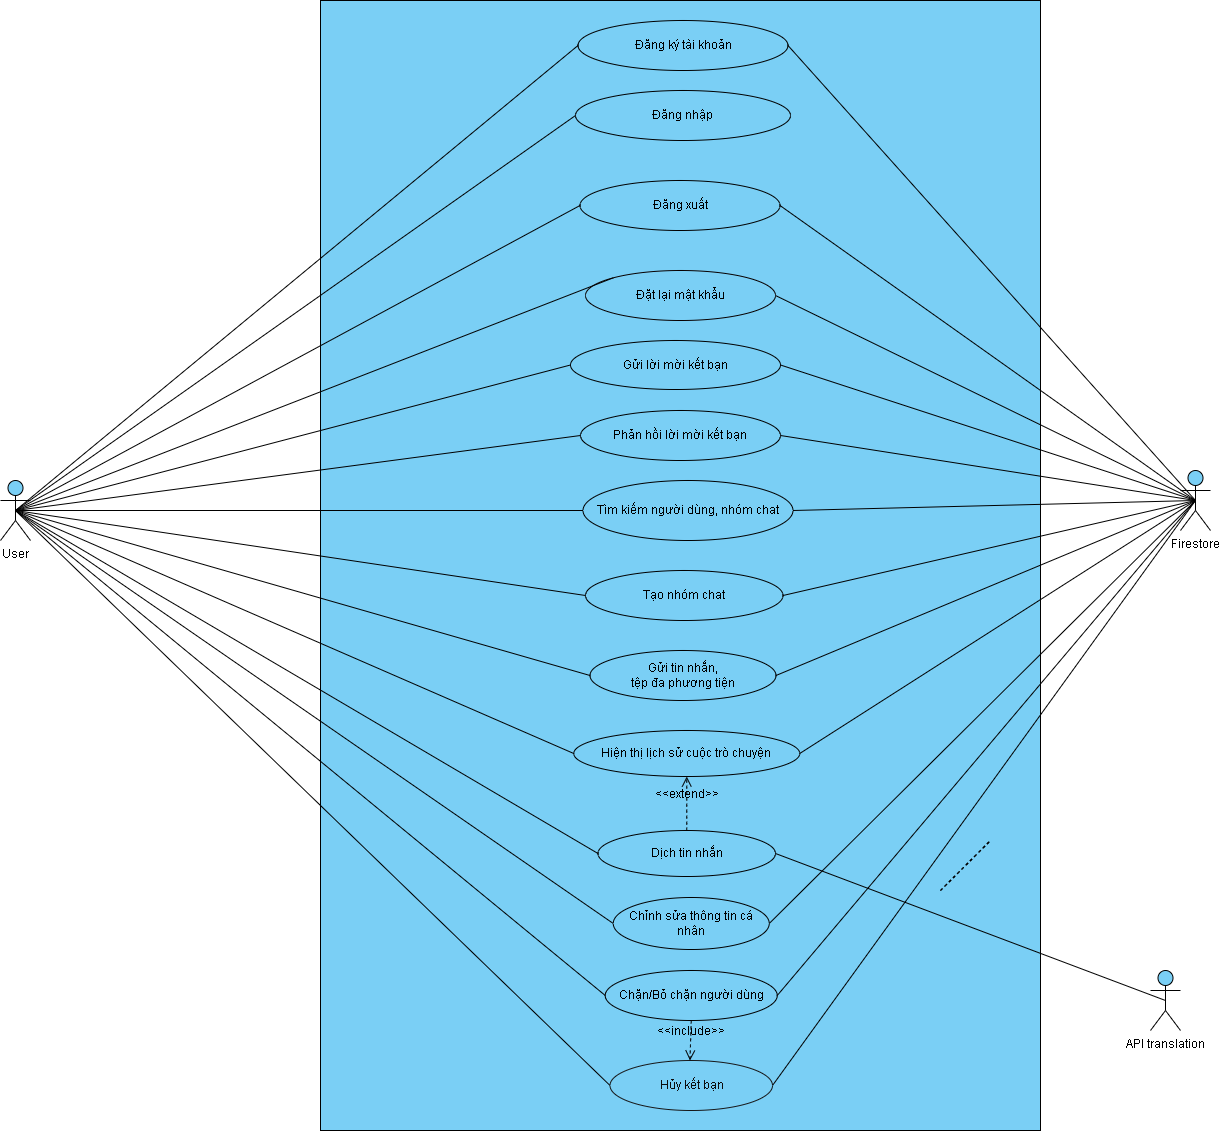
\includegraphics[width=1\textwidth]{UC tổng.drawio.png}    
		\caption{Sơ đồ Use-case tổng quát của hệ thống TransChat (\href{https://drive.google.com/file/d/1DxJgTyWZZEtigrcHEFEhs_xksvw2mR3u/view?usp=drive_link}{Xem ảnh gốc tại đây})}
		\label{fig:hinh-minh-hoa}
	\end{figure} 
	
	
	\newpage
	
	
	%%%%%%%%%%%%%%%%%%%%%%%%%%%%%%%
	%%%%% UC - Descriptions%%%%%%%%%
	%%%%%%%%%%%%%%%%%%%%%%%%%%%%%%%
	
	
	\subsection{Use Case Descriptions}
	
	\renewcommand{\arraystretch}{1.3}
	\setlist[enumerate]{nosep, leftmargin=*, label={[\arabic*]}}
	\setlist[itemize]{nosep, leftmargin=*, label={--}}
	
	% ======================================================================
	% U1 - Đăng ký
	% ======================================================================
	\begin{longtable}{|p{3.5cm}|p{12cm}|}
		\hline
		\textbf{Use-case ID} & 01 \\
		\hline
		\textbf{Use-case name} & Đăng ký tài khoản \\
		\hline
		\textbf{Actors} & User \\
		\hline
		\textbf{Description} & Cho phép người dùng mới tạo một tài khoản trong hệ thống bằng email, username và mật khẩu và xác thực Gmail. \\
		\hline
		\textbf{Trigger} & User nhấn vào nút "Đăng ký" trên màn hình đăng nhập. \\
		\hline
		\textbf{Precondition} & 
		\begin{itemize}[label=+]
			\item Người dùng chưa có tài khoản.
			\item Hệ thống đang hoạt động.
		\end{itemize} \\
		\hline
		\textbf{Postconditions} & Một document người dùng mới được tạo trong collection users trên Firestore với đầy đủ các trường mặc định và hệ thống thông báo đăng ký thành công. \\
		\hline
		\textbf{Normal flow} & 
		\begin{enumerate}
			\item Hệ thống hiển thị form đăng ký yêu cầu người dùng nhập: username, gmail, mật khẩu và xác nhận mật khẩu.
			\item Người dùng điền đầy đủ thông tin và nhấn nút "Đăng ký".
			\item Hệ thống kiểm tra tính hợp lệ của thông tin (username/gmail chưa tồn tại, mật khẩu trùng khớp).
			\item Nếu thông tin hợp lệ, hệ thống gửi một email xác thực tới địa chỉ Gmail mà người dùng cung cấp.
			\item Mã hóa (hash) mật khẩu của người dùng.
			\item Tạo một document mới trong collection users. Tên (ID) của document này là một ID người dùng duy nhất (UID) do hệ thống tạo ra.
			\item Khởi tạo document với các trường mặc định.
			\item Hệ thống thông báo đăng ký thành công và chuyển người dùng về màn hình đăng nhập.
		\end{enumerate} \\
		\hline
		\textbf{Exception flow} & 
		\begin{itemize}[label={}]
			\item \textbf{[2a]} Nếu username hoặc gmail đã tồn tại, hệ thống báo lỗi: "Tên người dùng hoặc Gmail đã tồn tại."
			\item \textbf{[2b]} Nếu mật khẩu xác nhận không khớp, hệ thống báo lỗi: "Mật khẩu không khớp."
			\item \textbf{[3a]} Nếu sau 30 phút mà tài khoản không được xác thực bằng gmail, đường link được gửi sẽ bị vô hiệu.
		\end{itemize} \\
		\hline
	\end{longtable}
	\vspace{0.5cm}
	
	% ======================================================================
	% U2 - Đăng nhập
	% ======================================================================
	\begin{longtable}{|p{3.5cm}|p{12cm}|}
		\hline
		\textbf{Use-case ID} & 02 \\
		\hline
		\textbf{Use-case name} & Đăng nhập vào hệ thống \\
		\hline
		\textbf{Actors} & User \\
		\hline
		\textbf{Description} & Cho phép người dùng đã có tài khoản truy cập vào ứng dụng bằng username và mật khẩu. \\
		\hline
		\textbf{Trigger} & Người dùng nhập thông tin và nhấn nút "Đăng nhập". \\
		\hline
		\textbf{Precondition} &  Người dùng đã có tài khoản.\\

		\hline
		\textbf{Postconditions} & Người dùng đăng nhập thành công. Trường status và session trong document của người dùng được cập nhật trên Firestore. \\
		\hline
		\textbf{Normal flow} & 
		\begin{enumerate}
			\item Người dùng nhập username và mật khẩu vào các trường tương ứng trên màn hình đăng nhập.
			\item Người dùng nhấn "Đăng nhập".
			\item Hệ thống tìm kiếm document trong collection users có trường username trùng khớp.
			\item Nếu tìm thấy, hệ thống so sánh mật khẩu người dùng nhập với trường hashed passwords đã lưu.
			\item Nếu xác thực thành công, hệ thống cập nhật document của người dùng tại users/\{userId\} (Set status 'online', cập nhật session).
			\item Hệ thống chuyển người dùng vào giao diện chính của ứng dụng.
		\end{enumerate} \\
		\hline
		\textbf{Exception flow} &  Nếu không tìm thấy username hoặc mật khẩu không đúng, hệ thống báo lỗi: "Sai tên đăng nhập hoặc mật khẩu."\\
		\hline
	\end{longtable}
	\vspace{0.5cm}
	
	% ======================================================================
	% U3 - Đăng xuất
	% ======================================================================
	\begin{longtable}{|p{3.5cm}|p{12cm}|}
		\hline
		\textbf{Use-case ID} & 03 \\
		\hline
		\textbf{Use-case name} & Đăng xuất khỏi hệ thống \\
		\hline
		\textbf{Actors} & User \\
		\hline
		\textbf{Description} & Cho phép người dùng đang đăng nhập có thể kết thúc phiên làm việc của mình. \\
		\hline
		\textbf{Trigger} & Người dùng chọn tùy chọn "Đăng xuất" trong menu cài đặt. \\
		\hline
		\textbf{Precondition} & Người dùng đang đăng nhập.\\
		\hline
		\textbf{Postconditions} & Người dùng đã được đăng xuất. Trường status được cập nhật thành 'offline'. \\
		\hline
		\textbf{Normal flow} & 
		\begin{enumerate}
			\item Người dùng nhấn nút "Đăng xuất".
			\item Hệ thống hiển thị hộp thoại xác nhận. Người dùng nhấn "Đồng ý".
			\item Hệ thống cập nhật document của người dùng: Set trường status thành 'offline'.
			\item Hệ thống xóa thông tin phiên đăng nhập trên thiết bị của người dùng.
			\item Hệ thống chuyển người dùng về màn hình đăng nhập.
		\end{enumerate} \\
		\hline
		\textbf{Exception flow} & Không có Exception. \\
		\hline
	\end{longtable}
	\vspace{0.5cm}
	
	% ======================================================================
	% U4 - Quên mật khẩu
	% ======================================================================
	\begin{longtable}{|p{3.5cm}|p{12cm}|}
		\hline
		\textbf{Use-case ID} & 04 \\
		\hline
		\textbf{Use-case name} & Đặt lại mật khẩu \\
		\hline
		\textbf{Actors} & User \\
		\hline
		\textbf{Description} & Cho phép người dùng đã quên mật khẩu có thể tạo một mật khẩu mới thông qua việc xác thực email (gmail). \\
		\hline
		\textbf{Trigger} & Người dùng nhấn vào đường dẫn "Quên mật khẩu?" trên màn hình đăng nhập. \\
		\hline
		\textbf{Precondition} & 
		\begin{itemize}[label=+]
			\item Người dùng nhớ được địa chỉ email đã dùng để đăng ký.
			\item Hệ thống có kết nối với dịch vụ gửi email.
		\end{itemize} \\
		\hline
		\textbf{Postconditions} & Mật khẩu được cập nhật an toàn. Người dùng có thể đăng nhập bằng mật khẩu mới. \\
		\hline
		\textbf{Normal flow} & 
		\begin{enumerate}
			\item Người dùng nhấn vào "Quên mật khẩu?".
			\item Hệ thống hiển thị màn hình yêu cầu nhập gmail.
			\item Người dùng nhập gmail và nhấn "Gửi yêu cầu".
			\item Hệ thống kiểm tra gmail trong collection users.
			\item Nếu tìm thấy, hệ thống tạo token tạm thời và gửi email chứa link xác thực.
			\item Người dùng mở mail và nhấp vào đường link.
			\item Người dùng nhập mật khẩu mới và xác nhận mật khẩu mới.
			\item Người dùng nhấn "Xác nhận".
			\item Hệ thống mã hóa mật khẩu mới và cập nhật vào CSDL.
			\item Hệ thống thông báo thành công và hướng người dùng về màn hình đăng nhập.
		\end{enumerate} \\
		\hline
		\textbf{Exception flow} & 
		\begin{itemize}[label={*}]
			\item Nếu gmail không tồn tại: Báo lỗi "Không tìm thấy tài khoản".
			\item Nếu link hết hạn/không hợp lệ: Yêu cầu thực hiện lại.
			\item Nếu mật khẩu xác nhận không khớp: Báo lỗi "Mật khẩu không khớp".
		\end{itemize} \\
		\hline
	\end{longtable}
	\vspace{0.5cm}
	
	% ======================================================================
	% U5 - Gửi lời mời kết bạn
	% ======================================================================
	\begin{longtable}{|p{3.5cm}|p{12cm}|}
		\hline
		\textbf{Use-case ID} & 05 \\
		\hline
		\textbf{Use-case name} & Gửi lời mời kết bạn \\
		\hline
		\textbf{Actors} & User \\
		\hline
		\textbf{Description} & Cho phép gửi lời mời kết bạn đến người dùng khác. \\
		\hline
		\textbf{Trigger} & Người dùng nhấn nút "Thêm bạn" trên trang cá nhân của người khác. \\
		\hline
		\textbf{Precondition} & 
		\begin{itemize}[label=+]
			\item Người dùng đã đăng nhập.
			\item ID người nhận chưa có trong danh sách bạn bè.
		\end{itemize} \\
		\hline
		\textbf{Postconditions} & Mảng friend\_request của người nhận chứa ID của người gửi. Trạng thái "Đã gửi lời mời" hiển thị. \\
		\hline
		\textbf{Normal flow} & 
		\begin{enumerate}
			\item Người dùng truy cập trang cá nhân của người muốn kết bạn.
			\item Người dùng nhấn "Thêm bạn".
			\item Hệ thống cập nhật Firestore: Thêm ID người gửi vào mảng friend\_request của người nhận.
			\item Hệ thống thông báo lời mời đã gửi thành công.
		\end{enumerate} \\
		\hline
		\textbf{Exception flow} & 
		\begin{itemize}[label={*}]
			\item Nếu đã gửi lời mời trước đó: Báo lỗi.
			\item Nếu bị chặn: Thông báo về việc bị chặn.
		\end{itemize} \\
		\hline
	\end{longtable}
	\vspace{0.5cm}
	
% ======================================================================
% U6 - Phản hồi lời mời kết bạn (Đã sửa đổi)
% ======================================================================
\begin{longtable}{|p{3.5cm}|p{12cm}|}
	\hline
	\textbf{Use-case ID} & U6. \\
	\hline
	\textbf{Use-case name} & Phản hồi lời mời kết bạn. \\
	\hline
	\textbf{Actors} & Người dùng (User). \\
	\hline
	\textbf{Description} & Cho phép người dùng chấp nhận hoặc từ chối một lời mời kết bạn. \\
	\hline
	\textbf{Trigger} & Người dùng vào danh sách lời mời kết bạn và nhấn "Chấp nhận" hoặc "Từ chối". \\
	\hline
	\textbf{Precondition} & 
	\begin{itemize}[nosep, leftmargin=*, label=+]
		\item Người dùng (người nhận) đã đăng nhập.
		\item Mảng friend\_request trong document của người nhận có chứa ít nhất một ID người gửi.
	\end{itemize} \\
	\hline
	\textbf{Post conditions} & 
	\begin{itemize}[nosep, leftmargin=*, label={-}]
		\item Khi chấp nhận: Hai người dùng trở thành bạn bè (ID của nhau xuất hiện trong mảng friends của nhau).
		\item Khi từ chối: Lời mời được xóa khỏi danh sách chờ (friend\_request).
	\end{itemize} \\
	\hline
	\textbf{Normal flow} & 
	[1] Người dùng truy cập trang quản lý lời mời kết bạn. \newline
	[2] Giao diện đọc mảng friend\_request để hiển thị danh sách người gửi lời mời. \newline
	[3] Người dùng chọn một lời mời và thực hiện hành động: \newline
	\textbf{Luồng A - Chấp nhận:} \newline
	[A1] Người dùng nhấn "Chấp nhận". \newline
	[A2] Hệ thống thực hiện 3 thao tác cập nhật trên Firestore:
	\begin{itemize}[nosep, leftmargin=0.5cm, label={}]
		\item a. Cập nhật người nhận: Thêm ID người gửi vào mảng friends.
		\item b. Cập nhật người gửi: Tìm đến document users/\{senderId\} và thêm ID người nhận vào mảng friends.
		\item c. Dọn dẹp lời mời: Xóa ID người gửi khỏi mảng friend\_request của người nhận.
	\end{itemize}
	\textbf{Luồng B - Từ chối:} \newline
	[B1] Người dùng nhấn "Từ chối". \newline
	[B2] Hệ thống cập nhật document của người nhận: Xóa ID người gửi khỏi mảng friend\_request. \\
	\hline
	\textbf{Exceptions} & Nếu có lỗi xảy ra trong quá trình cập nhật 2 chiều (ví dụ người gửi đã xóa tài khoản), hệ thống sẽ cố gắng hoàn tác giao dịch và báo lỗi. \\
	\hline
\end{longtable}
\vspace{0.5cm}
	
	% ======================================================================
	% U7 - Tìm kiếm (Đã sửa đổi)
	% ======================================================================
	\begin{longtable}{|p{3.5cm}|p{12cm}|}
		\hline
		\textbf{Use-case ID} & U7. \\
		\hline
		\textbf{Use-case name} & Tìm kiếm người dùng, nhóm chat. \\
		\hline
		\textbf{Actors} & Người dùng (User). \\
		\hline
		\textbf{Description} & Cho phép người dùng tìm kiếm người dùng (theo username hoặc gmail) và nhóm chat (theo chat\_name). Hệ thống chuẩn hoá từ khoá, truy vấn, lọc và hiển thị kết quả. \\
		\hline
		\textbf{Trigger} & Người dùng nhập một từ khóa vào thanh tìm kiếm chính của ứng dụng. \\
		\hline
		\textbf{Precondition} & Người dùng đã đăng nhập vào hệ thống. \\
		\hline
		\textbf{Post conditions} & Một danh sách người dùng hoặc nhóm phù hợp với từ khóa tìm kiếm được hiển thị cho người dùng. \\
		\hline
		\textbf{Normal flow} & 
		[1] Người dùng nhập username, gmail hoặc chat\_name vào thanh tìm kiếm. \newline
		[2] Hệ thống chuẩn hoá đầu vào: trim khoảng trắng, chuyển thường, bỏ dấu tiếng Việt. \newline
		[3] Hệ thống thực hiện truy vấn trên collection users và collection chat (loại group):
		\begin{itemize}[nosep, leftmargin=0.5cm, label={-}]
			\item Tìm các document có trường username hoặc gmail trùng khớp chính xác.
			\item Tìm các chat có chat\_name trùng khớp.
		\end{itemize}
		[4] Hệ thống trả về danh sách các document phù hợp. \newline
		[5] Giao diện hiển thị danh sách kết quả (bao gồm Avatar và Tên). \newline
		[6] Người dùng có thể nhấn vào một kết quả để xem trang cá nhân hoặc tham gia nhóm. \\
		\hline
		\textbf{Exceptions} & 
		[3a] Nếu không tìm thấy document nào khớp, hệ thống hiển thị thông báo: "Không tìm thấy". \newline
		[3b] Nếu người dùng tìm thấy nằm trong danh sách chặn, kết quả đó sẽ bị ẩn đi. \newline
		[3c] Nếu có lỗi kết nối mạng trong quá trình truy vấn, hệ thống sẽ báo lỗi. \\
		\hline
	\end{longtable}
	\vspace{0.5cm}
	
	% ======================================================================
	% U8 - Tạo nhóm chat (Đã sửa đổi)
	% ======================================================================
	\begin{longtable}{|p{3.5cm}|p{12cm}|}
		\hline
		\textbf{Use-case ID} & U8. \\
		\hline
		\textbf{Use-case name} & Tạo nhóm chat. \\
		\hline
		\textbf{Actors} & User. \\
		\hline
		\textbf{Description} & Cho phép người dùng tạo một cuộc trò chuyện nhóm mới, đặt tên cho nhóm và mời các thành viên từ danh sách bạn bè. \\
		\hline
		\textbf{Trigger} & Người dùng nhấn vào nút "Tạo nhóm mới" trên giao diện danh sách trò chuyện. \\
		\hline
		\textbf{Precondition} & 
		\begin{itemize}[nosep, leftmargin=*, label=+]
			\item Người dùng đã đăng nhập.
			\item Người dùng có ít nhất một người bạn để có thể tạo nhóm.
		\end{itemize} \\
		\hline
		\textbf{Post conditions} & 
		\begin{itemize}[nosep, leftmargin=*, label={-}]
			\item Một collection trò chuyện nhóm mới được tạo thành công trên Firestore.
			\item Tất cả các thành viên được mời đều có quyền truy cập vào nhóm chat này.
		\end{itemize} \\
		\hline
		\textbf{Normal flow} & 
		[1] Người dùng nhấn nút "Tạo nhóm mới". \newline
		[2] Hệ thống hiển thị giao diện nhập tên nhóm và danh sách bạn bè để chọn. \newline
		[3] Người dùng nhập tên nhóm và chọn ít nhất một người bạn. \newline
		[4] Người dùng nhấn nút "Tạo". \newline
		[5] Hệ thống thực hiện các thao tác sau trên Firestore: \newline
		\hspace*{0.5cm} [5.1] Tạo một collection mới bên trong chat với một ID duy nhất. \newline
		\hspace*{0.5cm} [5.2] Tạo document metadata có ID là -1 bên trong collection này. \newline
		\hspace*{0.5cm} [5.3] Điền thông tin vào document metadata: type: 'group', chat\_name, date created, và mảng nickname chứa thông tin các thành viên. \newline
		[6] Hệ thống tự động chuyển người dùng vào màn hình trò chuyện của nhóm vừa tạo. \\
		\hline
		\textbf{Exceptions} & [4a] Nếu người dùng không nhập tên nhóm hoặc không chọn thành viên nào, hệ thống hiển thị lỗi và không cho phép tạo. \\
		\hline
	\end{longtable}
	\vspace{0.5cm}
	
	% ======================================================================
	% U9 - Tui chưa thấy
	% ======================================================================
	
	
	% ======================================================================
	% U10 - Gửi tin nhắn
	% ======================================================================
	\begin{longtable}{|p{3.5cm}|p{12cm}|}
		\hline
		\textbf{Use-case ID} & 10 \\
		\hline
		\textbf{Use-case name} & Gửi tin nhắn và tệp đa phương tiện \\
		\hline
		\textbf{Actors} & Người dùng (User) \\
		\hline
		\textbf{Description} & Gửi tin nhắn văn bản hoặc tệp đa phương tiện (ảnh, video). \\
		\hline
		\textbf{Trigger} & Nhấn nút "Gửi" hoặc chọn tệp đính kèm. \\
		\hline
		\textbf{Precondition} & 
		\begin{itemize}[label=+, leftmargin=1.5em] 
			\item Người dùng đã đăng nhập.
			\item Người dùng đang ở màn hình một cuộc trò chuyện.
		\end{itemize} \\
		\hline
		\textbf{Postconditions} & 
		\begin{itemize}[label=+, leftmargin=1.5em]
			\item Document tin nhắn được lưu vào Database.
			\item Nếu là tệp đa phương tiện: tệp gốc lưu trên Cloud và document trên Database chứa URL của tệp này.
		\end{itemize} \\
		\hline
		\textbf{Normal Flows} & 
		\begin{enumerate}[leftmargin=1.5em] 
			\item Người dùng nhập văn bản xong nhấn “Gửi”.
			\item Hệ thống tạo document mới trong \texttt{chat/\{chatId\}}.
			\item Tin nhắn hiển thị ngay trên giao diện người gửi và đồng bộ tới thành viên khác.
		\end{enumerate} \\
		\hline
		\textbf{Alternative Flows} & 
		\begin{itemize}[leftmargin=3em, labelsep=0.5em] 
			\item[1.1.] Người dùng chọn ảnh/video rồi xác nhận gửi.
			\item[1.2.] Hệ thống tải tệp lên Cloud.
			\item[1.3.] Nếu tải lên thành công, nhận URL của tệp rồi tạo document mới trong \texttt{chat/\{chatId\}} và chứa URL của tệp.
			\item[1.4.] Giao diện hiển thị preview (thumbnail) và đồng bộ tin nhắn tới thành viên khác.
		\end{itemize} \\
		\hline
		\textbf{Exception Flows} & 
		\begin{itemize}[leftmargin=3.5em, labelsep=0.5em]
			\item[1.1.1.] File > 4MB thì hệ thống từ chối, hiển thị cảnh báo “File gửi đi không được quá 4MB”.
			\item[1.2.1.] Tải lên Cloud thất bại, hệ thống thông báo lỗi gửi tệp cho người dùng, không tạo document.
		\end{itemize} \\
		\hline
	\end{longtable}
	\vspace{0.5cm}
	
	% ======================================================================
	% U11 - Lịch sử chat
	% ======================================================================
	\begin{longtable}{|p{3.5cm}|p{12cm}|}
		\hline
		\textbf{Use-case ID} & 11 \\
		\hline
		\textbf{Use-case name} & Hiển thị lịch sử trò chuyện \\
		\hline
		\textbf{Actors} & Người dùng (User) \\
		\hline
		\textbf{Description} & Cho phép người dùng xem toàn bộ lịch sử tin nhắn trong một cuộc trò chuyện. \\
		\hline
		\textbf{Trigger} & Người dùng mở một cuộc trò chuyện từ danh sách chat. \\
		\hline
		\textbf{Precondition} & Người dùng đã đăng nhập. \\
		\hline
		\textbf{Postconditions} & Người dùng có thể cuộn xem tin nhắn cũ; ảnh/video có thể xem trực tiếp. \\
		\hline
		\textbf{Normal Flows} & 
		\begin{enumerate}[leftmargin=1.5em]
			\item Người dùng chọn mở cuộc trò chuyện.
			\item Hệ thống truy vấn \texttt{chat/\{chatId\}} và lấy các document, sắp xếp theo \texttt{timestamp} tăng dần.
			\item Hệ thống lặp qua từng document và hiển thị nội dung lên giao diện.
			\item Hệ thống đọc giá trị từ trường nội dung tin nhắn.
			\item Nếu là tin nhắn văn bản $\rightarrow$ hiển thị dưới dạng bong bóng chat văn bản.
		\end{enumerate} \\
		\hline
		\textbf{Alternative Flows} & 
		\begin{itemize}[leftmargin=2.5em, labelsep=0.5em]
			\item[4.1.] Nếu là tệp đa phương tiện:
			\item[4.2.] Hệ thống đọc giá trị URL từ trường nội dung tin nhắn.
			\item[4.3.] Nếu là ảnh/video $\rightarrow$ hiển thị thumbnail; người dùng có thể nhấn để stream trực tiếp từ URL. (Ứng dụng dùng URL stream full độ phân giải mà không cần tải về trước).
			\item[4.4.] Nếu là tệp khác $\rightarrow$ chỉ hiển thị URL.
		\end{itemize} \\
		\hline
		\textbf{Exception Flows} & 
		\begin{itemize}[leftmargin=3.5em, labelsep=0.5em]
			\item[4.1.1.] URL tệp không còn hợp lệ (tệp đã xóa trên Cloud) $\rightarrow$ hiển thị thông báo lỗi hoặc biểu tượng tệp hỏng.
		\end{itemize} \\
		\hline
	\end{longtable}
	\vspace{0.5cm}
	
	% ======================================================================
	% U12 - Dịch tin nhắn
	% ======================================================================
	\begin{longtable}{|p{3.5cm}|p{12cm}|}
		\hline
		\textbf{Use-case ID} & 12 \\
		\hline
		\textbf{Use-case name} & Dịch tin nhắn \\
		\hline
		\textbf{Actors} & Người dùng (User) \\
		\hline
		\textbf{Description} & Cho phép người dùng dịch toàn bộ tin nhắn văn bản trong một cuộc trò chuyện (hiển thị bản dịch song song với nội dung gốc hoặc ẩn nội dung gốc). \\
		\hline
		\textbf{Trigger} & Người dùng vào cài đặt của cuộc trò chuyện và chọn “Dịch tin nhắn”. \\
		\hline
		\textbf{Precondition} & Người dùng đang ở trong một cuộc trò chuyện. \\
		\hline
		\textbf{Postconditions} & Giao diện hiển thị bản dịch cho các tin nhắn văn bản; người dùng có thể xem bản gốc song song hoặc ẩn bản gốc. \\
		\hline
		\textbf{Normal Flows} & 
		\begin{enumerate}[leftmargin=1.5em]
			\item Người dùng chọn “Dịch tin nhắn”.
			\item Hệ thống truy vấn các document trong \texttt{chat/\{chatId\}} (các tin nhắn văn bản).
			\item Hệ thống nhận về danh sách document tin nhắn văn bản.
			\item Hệ thống gọi API Translation để dịch trường nội dung của các tin nhắn.
			\item Hệ thống nhận kết quả dịch và trả về nội dung đã dịch, giao diện hiển thị bản dịch song song với bản gốc.
		\end{enumerate} \\
		\hline
		\textbf{Alternative Flows} & 
		\begin{itemize}[leftmargin=2.5em, labelsep=0.5em]
			\item[5.1.] Nếu chọn ẩn bản dịch $\rightarrow$ không hiển thị bản dịch. Có thể mở lại bản dịch.
		\end{itemize} \\
		\hline
		\textbf{Exception Flows} & Lỗi kết nối API Translation (Hệ thống không thể kết nối tới dịch vụ dịch thuật). \\
		\hline
	\end{longtable}
	\vspace{0.5cm}
	
	% ======================================================================
	% U13 - Chỉnh sửa Profile
	% ======================================================================
	\begin{longtable}{|p{3.5cm}|p{12cm}|}
		\hline
		\textbf{Use-case ID} & 13 \\
		\hline
		\textbf{Use-case name} & Chỉnh sửa thông tin cá nhân \\
		\hline
		\textbf{Actors} & User \\
		\hline
		\textbf{Description} & Cập nhật ảnh đại diện và thông tin bio/status. \\
		\hline
		\textbf{Trigger} & Nhấn nút "Chỉnh sửa hồ sơ" trên trang cá nhân. \\
		\hline
		\textbf{Precondition} & 
		\begin{itemize}[label=+]
			\item Người dùng đã đăng nhập.
		\end{itemize} \\
		\hline
		\textbf{Postconditions} & Profile được cập nhật trên Firestore và hiển thị mới trên ứng dụng. \\
		\hline
		\textbf{Normal flow} & 
		\begin{enumerate}
			\item Người dùng điều hướng đến trang cá nhân, nhấn "Chỉnh sửa".
			\item[] \textbf{Thay đổi Avatar:}
			\item Người dùng chọn ảnh từ thư viện.
			\item Hệ thống upload lên Drive, lấy URL mới.
			\item[] \textbf{Thay đổi Bio:}
			\item Người dùng nhập nội dung mới.
			\item Người dùng nhấn "Lưu".
			\item Hệ thống cập nhật document users (URL avatar, profiles).
			\item Hệ thống thông báo thành công và làm mới giao diện.
		\end{enumerate} \\
		\hline
		\textbf{Exception flow} & 
		\begin{itemize}[label={*}]
			\item Upload ảnh thất bại: Báo lỗi.
			\item Thông tin không hợp lệ: Cảnh báo.
		\end{itemize} \\
		\hline
	\end{longtable}
	\vspace{0.5cm}
	
	% ======================================================================
	% U14 - Xóa bạn
	% ======================================================================
	\begin{longtable}{|p{3.5cm}|p{12cm}|}
		\hline
		\textbf{Use-case ID} & 14 \\
		\hline
		\textbf{Use-case name} & Xóa bạn (Hủy kết bạn) \\
		\hline
		\textbf{Actors} & User \\
		\hline
		\textbf{Description} & Gỡ bỏ một người dùng khỏi danh sách bạn bè (hai chiều). \\
		\hline
		\textbf{Trigger} & Chọn "Xóa bạn" trên trang cá nhân bạn bè. \\
		\hline
		\textbf{Precondition} & 
		\begin{itemize}[label=+]
			\item Hai người dùng đang là bạn bè.
		\end{itemize} \\
		\hline
		\textbf{Postconditions} & Mối quan hệ bạn bè bị xóa khỏi CSDL. \\
		\hline
		\textbf{Normal flow} & 
		\begin{enumerate}
			\item Người dùng truy cập trang cá nhân của bạn bè, chọn "Xóa bạn".
			\item Hệ thống hỏi xác nhận. Người dùng nhấn "Xác nhận".
			\item Hệ thống thực hiện transaction cập nhật Firestore:
			\item Gỡ bỏ ID bạn khỏi mảng friends của người dùng.
			\item Gỡ bỏ ID người dùng khỏi mảng friends của bạn.
			\item Cập nhật giao diện, xóa khỏi danh sách hiển thị.
		\end{enumerate} \\
		\hline
		\textbf{Exception flow} & Lỗi kết nối/transaction: Báo lỗi để đảm bảo tính nhất quán dữ liệu. \\
		\hline
	\end{longtable}
	\vspace{0.5cm}
	
	% ======================================================================
	% U15 - Chặn người dùng
	% ======================================================================
	\begin{longtable}{|p{3.5cm}|p{12cm}|}
		\hline
		\textbf{Use-case ID} & 15 \\
		\hline
		\textbf{Use-case name} & Chặn/Bỏ chặn người dùng \\
		\hline
		\textbf{Actors} & User \\
		\hline
		\textbf{Description} & Ngăn chặn người dùng khác tương tác (nhắn tin, kết bạn). \\
		\hline
		\textbf{Trigger} & Chọn "Chặn" trên trang cá nhân người khác. \\
		\hline
		\textbf{Precondition} & 
		\begin{itemize}[label=+]
			\item Người dùng đã đăng nhập.
		\end{itemize} \\
		\hline
		\textbf{Postconditions} & ID người bị chặn vào danh sách blocked\_users (hoặc ngược lại). \\
		\hline
		\textbf{Normal flow} & 
		\begin{enumerate}
			\item Người dùng truy cập trang cá nhân đối phương.
			\item[] \textbf{Trường hợp Chặn:}
			\item Chọn "Chặn", xác nhận hộp thoại.
			\item Hệ thống thêm ID đối phương vào mảng blocked\_users.
			\item Nếu đang là bạn bè: Tự động gọi quy trình Xóa bạn (U14).
			\item Hệ thống thông báo chặn thành công.
			\item[] \textbf{Trường hợp Bỏ chặn:}
			\item Chọn "Bỏ chặn", xác nhận hộp thoại.
			\item Hệ thống xóa ID đối phương khỏi mảng blocked\_users.
		\end{enumerate} \\
		\hline
		\textbf{Exception flow} &  Chặn chính mình: Giao diện ẩn tùy chọn này.\\
		\hline
	\end{longtable}
	
	%%%%%%%%%%%%%%%%%%%%%%%%%%%%%
	%%%%% System Modeling %%%%%%%
	%%%%%%%%%%%%%%%%%%%%%%%%%%%%%
	
	\section{System Modeling}
	\subsection{Activity Diagrams}
	
	%Tui nghĩ là nên các AD chính thôi để tránh báo cáo dài, mà tôi đưa hết để mn tiện 
	%Tui không có hình gốc một số UC nên hơi vỡ mn thay vào nha
	
	% --- UC01 ---
	\subsubsection*{UC01: Đăng ký tài khoản}
	\begin{figure}[H]
		\centering
		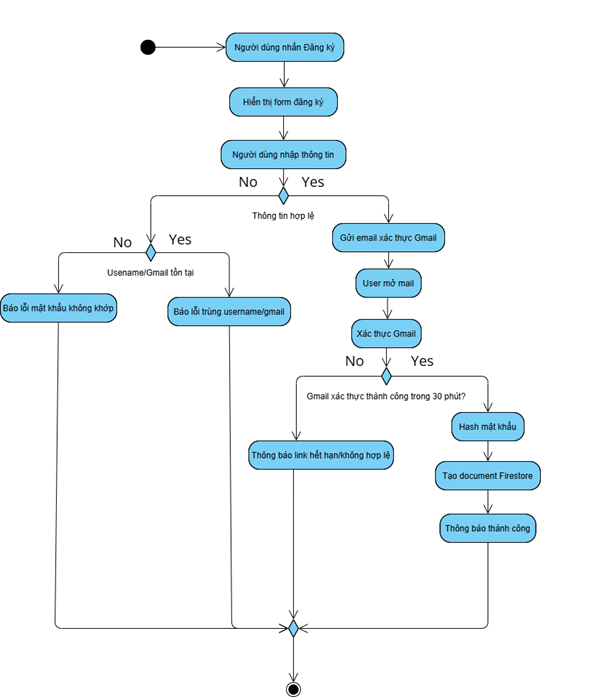
\includegraphics[width=0.8\textwidth]{Images/ActivityDiagram/U1.png}
		\caption{Activity Diagram: Quy trình Đăng ký tài khoản}
		\label{fig:act_uc01}
	\end{figure}
	
	% --- UC02 ---
	\subsubsection*{UC02: Đăng nhập vào hệ thống}
	\begin{figure}[H]
		\centering
		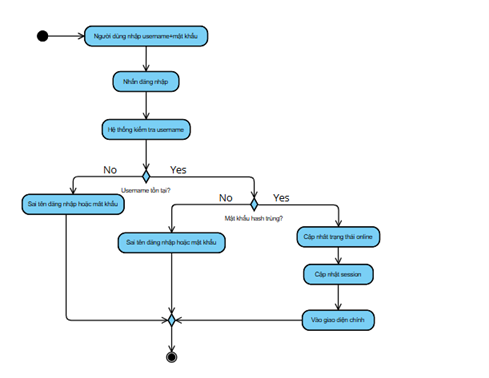
\includegraphics[width=0.8\textwidth]{Images/ActivityDiagram/U2.png}
		\caption{Activity Diagram: Quy trình Đăng nhập}
		\label{fig:act_uc02}
	\end{figure}
	
	% --- UC03 ---
	\subsubsection*{UC03: Đăng xuất khỏi hệ thống}
	\begin{figure}[H]
		\centering
		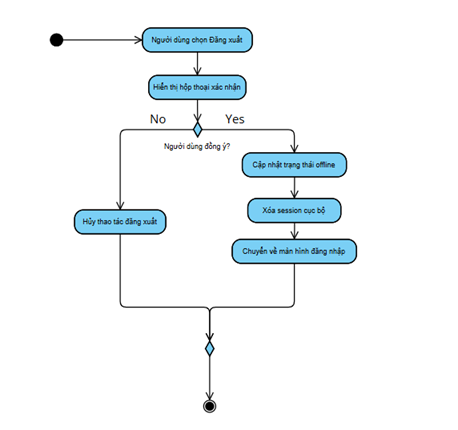
\includegraphics[width=0.8\textwidth]{Images/ActivityDiagram/U3.png}
		\caption{Activity Diagram: Quy trình Đăng xuất}
		\label{fig:act_uc03}
	\end{figure}
	
	% --- UC04 ---
	\subsubsection*{UC04: Đặt lại mật khẩu}
	\begin{figure}[H]
		\centering
		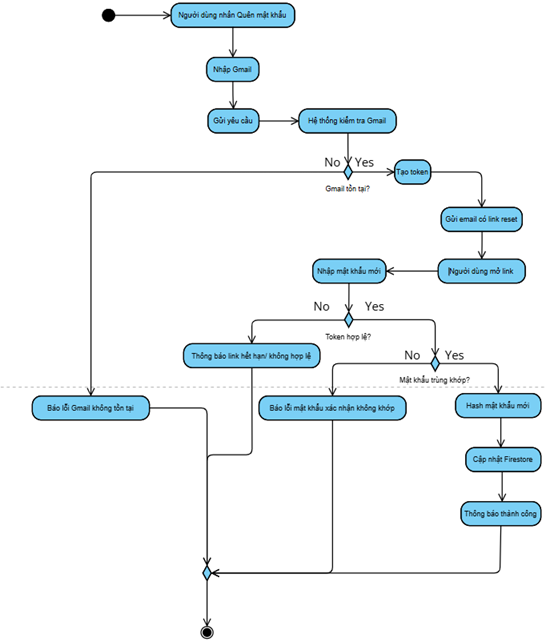
\includegraphics[width=0.8\textwidth]{Images/ActivityDiagram/U4.png}
		\caption{Activity Diagram: Quy trình Đặt lại mật khẩu}
		\label{fig:act_uc04}
	\end{figure}
	
	% --- UC05 ---
	\subsubsection*{UC05: Gửi lời mời kết bạn}
	\begin{figure}[H]
		\centering
		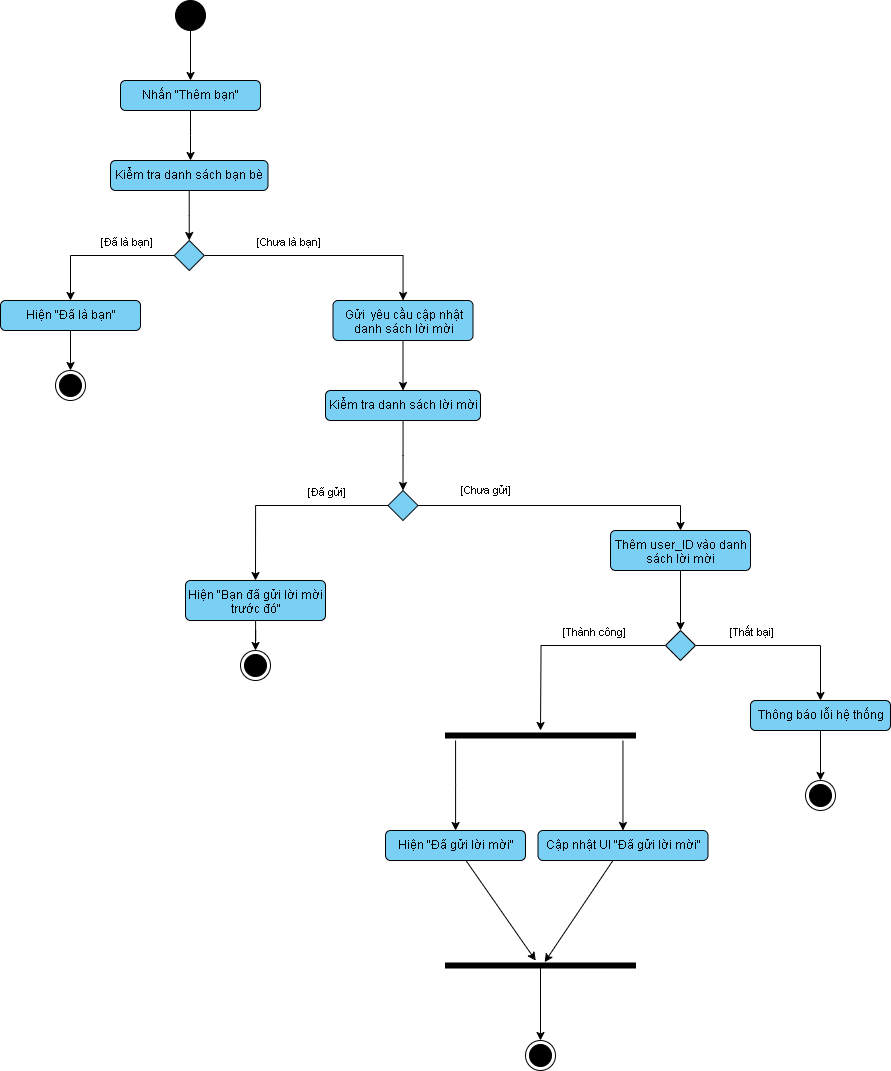
\includegraphics[width=0.8\textwidth]{Images/ActivityDiagram/U5.png}
		\caption{Activity Diagram: Quy trình Gửi lời mời kết bạn}
		\label{fig:act_uc05}
	\end{figure}
	
	% --- UC06 ---
	\subsubsection*{UC06: Phản hồi lời mời kết bạn}
	\begin{figure}[H]
		\centering
		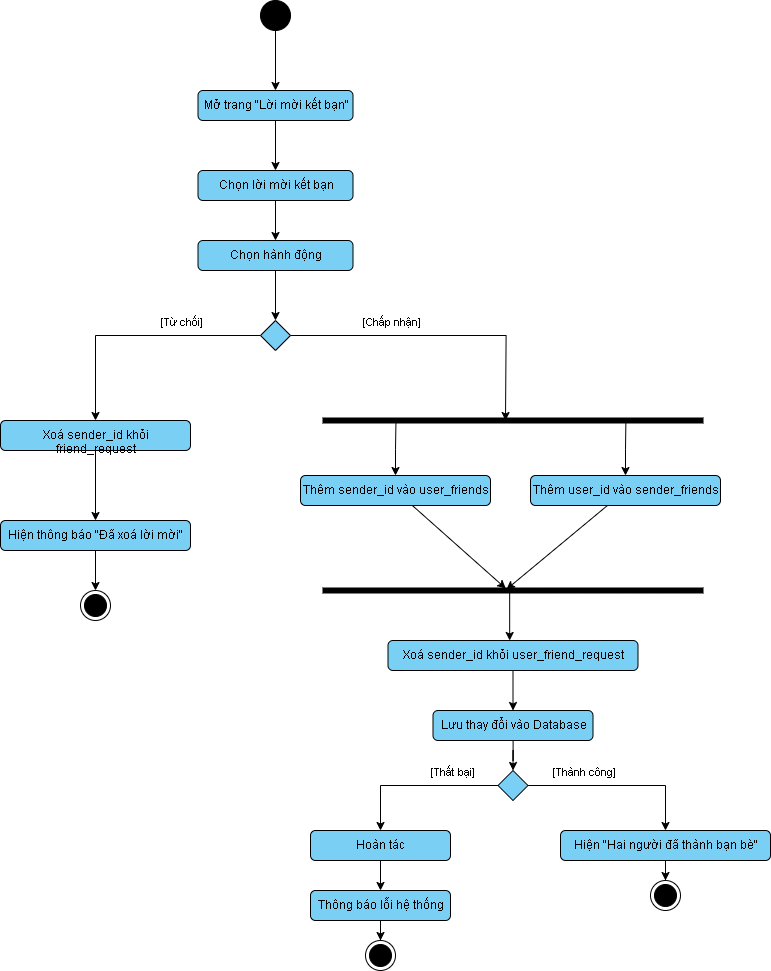
\includegraphics[width=0.8\textwidth]{Images/ActivityDiagram/U6.png}
		\caption{Activity Diagram: Quy trình Phản hồi kết bạn}
		\label{fig:act_uc06}
	\end{figure}
	
	% --- UC07 ---
	\subsubsection*{UC07: Tìm kiếm người dùng, nhóm chat}
	\begin{figure}[H]
		\centering
		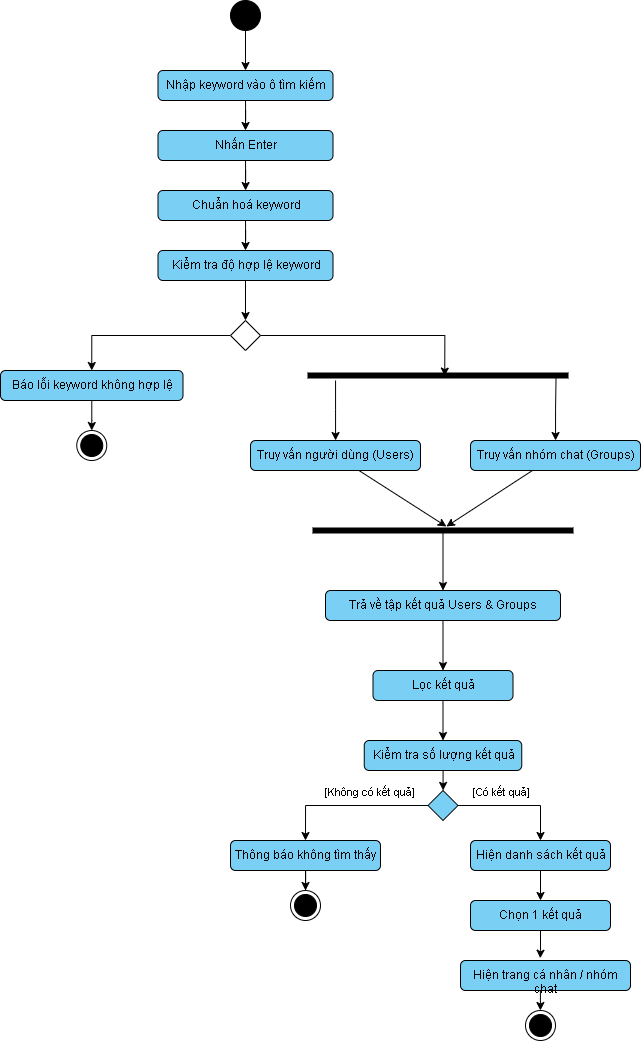
\includegraphics[width=0.8\textwidth]{Images/ActivityDiagram/U7.png}
		\caption{Activity Diagram: Quy trình Tìm kiếm}
		\label{fig:act_uc07}
	\end{figure}
	
	% --- UC08 ---
	\subsubsection*{UC08: Tạo nhóm chat}
	\begin{figure}[H]
		\centering
		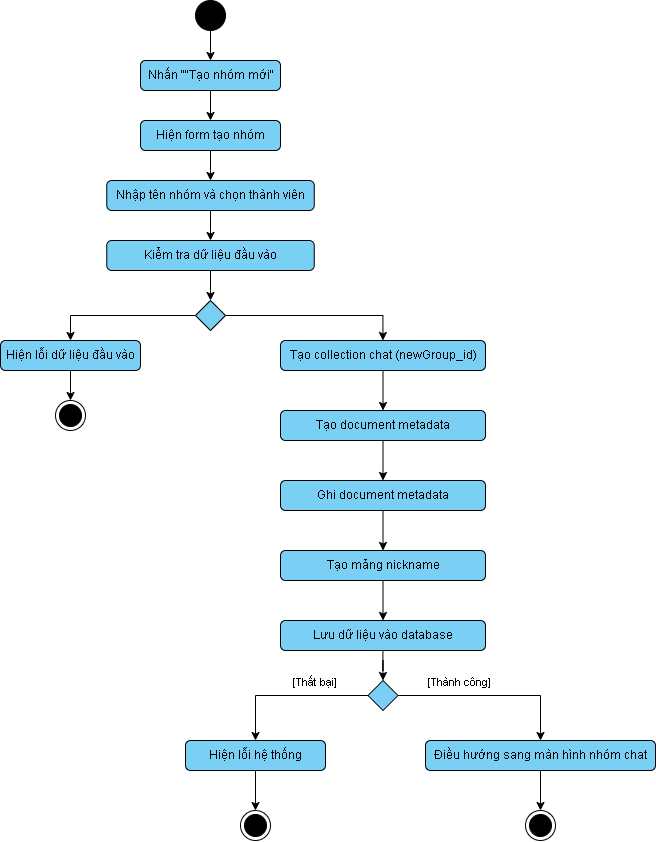
\includegraphics[width=0.8\textwidth]{Images/ActivityDiagram/U8.png}
		\caption{Activity Diagram: Quy trình Tạo nhóm chat}
		\label{fig:act_uc08}
	\end{figure}
	
	% --- UC10  ---
	\subsubsection*{UC10: Gửi tin nhắn và tệp đa phương tiện}
	\begin{figure}[H]
		\centering
		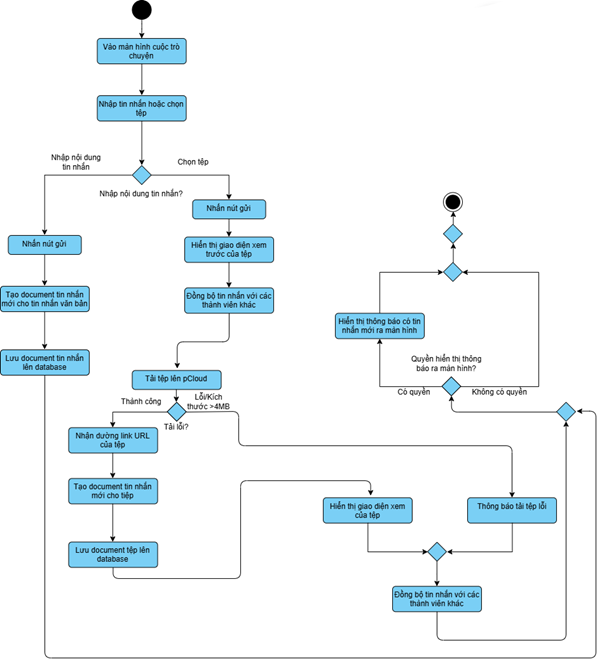
\includegraphics[width=0.8\textwidth]{Images/ActivityDiagram/U10.png}
		\caption{Activity Diagram: Quy trình Gửi tin nhắn}
		\label{fig:act_uc10}
	\end{figure}
	
	% --- UC11 ---
	\subsubsection*{UC11: Hiển thị lịch sử trò chuyện}
	\begin{figure}[H]
		\centering
		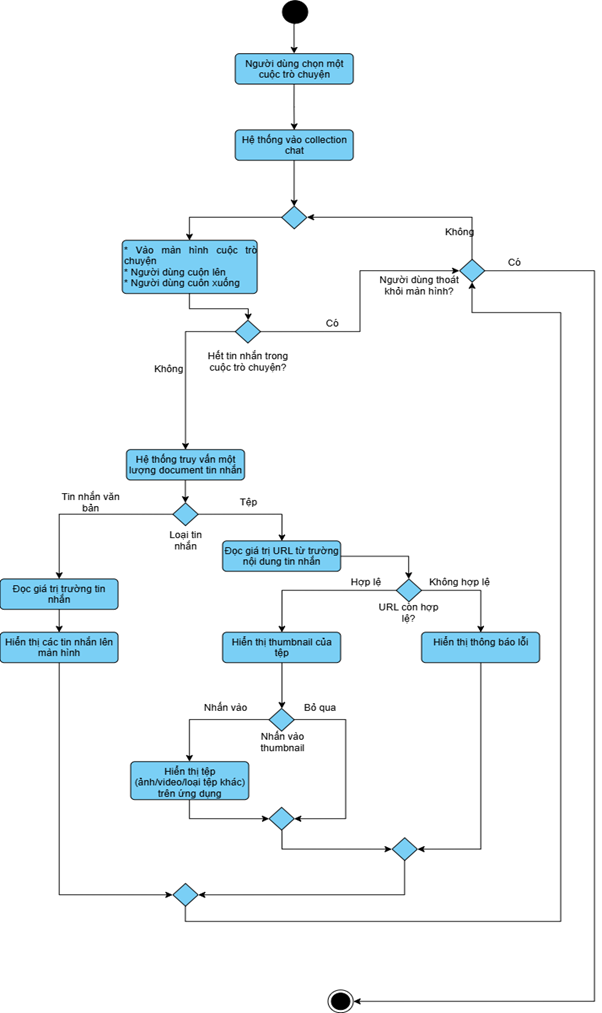
\includegraphics[width=0.8\textwidth]{Images/ActivityDiagram/U11.png}
		\caption{Activity Diagram: Quy trình Hiển thị lịch sử chat}
		\label{fig:act_uc11}
	\end{figure}
	
	% --- UC12 ---
	\subsubsection*{UC12: Dịch tin nhắn}
	\begin{figure}[H]
		\centering
		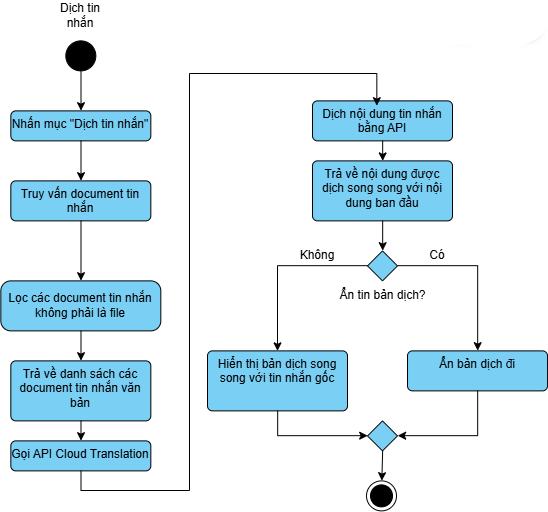
\includegraphics[width=0.8\textwidth]{Images/ActivityDiagram/U12.png}
		\caption{Activity Diagram: Quy trình Dịch tin nhắn}
		\label{fig:act_uc12}
	\end{figure}
	
	% --- UC13 ---
	\subsubsection*{UC13: Chỉnh sửa thông tin cá nhân}
	\begin{figure}[H]
		\centering
		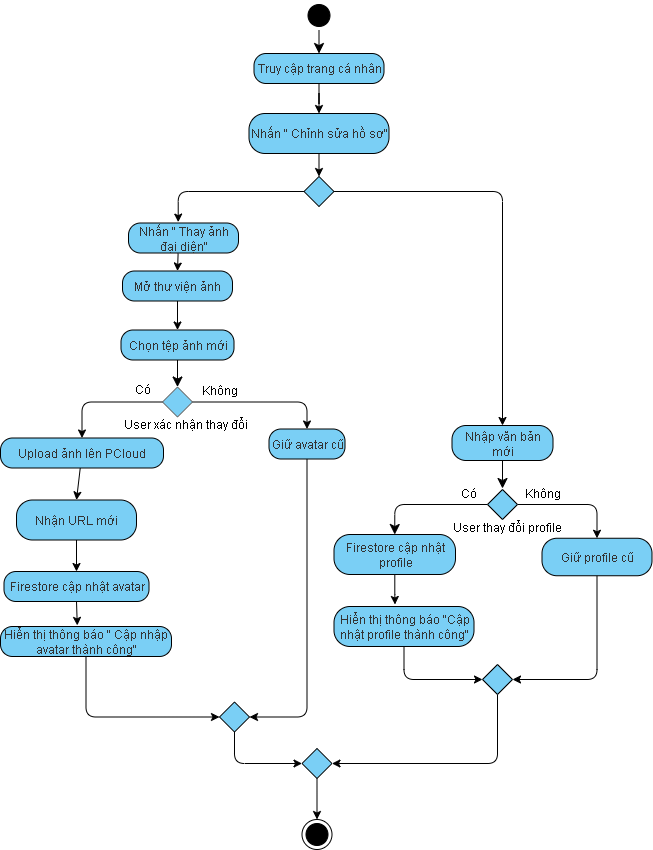
\includegraphics[width=0.8\textwidth]{Images/ActivityDiagram/U13.png}
		\caption{Activity Diagram: Quy trình Chỉnh sửa hồ sơ}
		\label{fig:act_uc13}
	\end{figure}
	
	% --- UC14 ---
	\subsubsection*{UC14: Xóa bạn (Hủy kết bạn)}
	\begin{figure}[H]
		\centering
		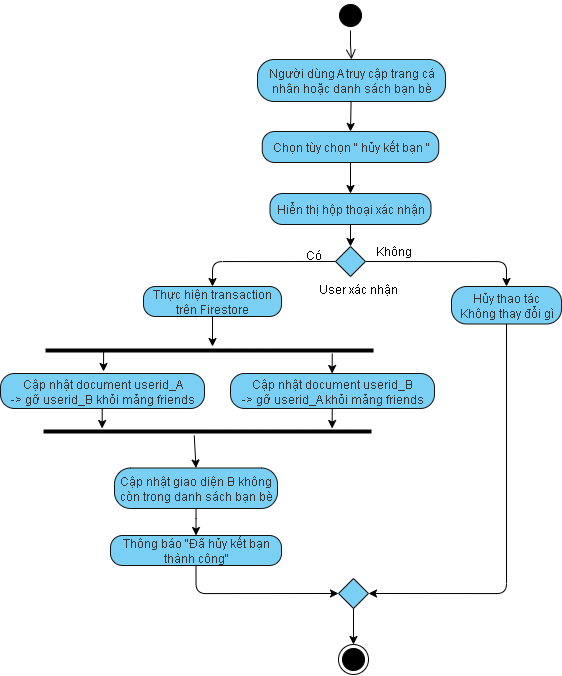
\includegraphics[width=0.8\textwidth]{Images/ActivityDiagram/U14.png}
		\caption{Activity Diagram: Quy trình Hủy kết bạn}
		\label{fig:act_uc14}
	\end{figure}
	
	% --- UC15 ---
	\subsubsection*{UC15: Chặn/Bỏ chặn người dùng}
	\begin{figure}[H]
		\centering
		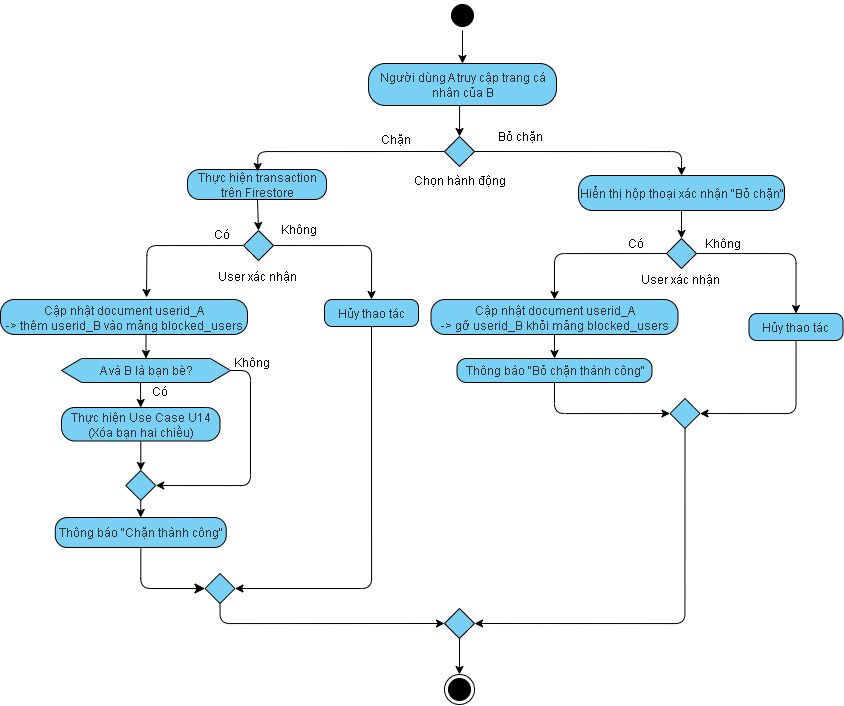
\includegraphics[width=0.8\textwidth]{Images/ActivityDiagram/U15.png}
		\caption{Activity Diagram: Quy trình Chặn và Bỏ chặn}
		\label{fig:act_uc15}
	\end{figure}
	
	\newpage
	\subsection{Sequence Diagrams}
	
	%Cái này cũng z nha
	
	% --- UC01 ---
	\subsubsection*{UC01: Đăng ký tài khoản}
	\begin{figure}[H]
		\centering
		
\includegraphics[width=0.8\textwidth]{Images/SequenceDiagram/U1.png}
		\caption{Sequence Diagram: Đăng ký tài khoản}
		\label{fig:seq_uc01}
	\end{figure}
	
	% --- UC02 ---
	\subsubsection*{UC02: Đăng nhập vào hệ thống}
	\begin{figure}[H]
		\centering
		
\includegraphics[width=0.8\textwidth]{Images/SequenceDiagram/U2.png}
		\caption{Sequence Diagram: Đăng nhập}
		\label{fig:seq_uc02}
	\end{figure}
	
	% --- UC03 ---
	\subsubsection*{UC03: Đăng xuất khỏi hệ thống}
	\begin{figure}[H]
		\centering
		
\includegraphics[width=0.8\textwidth]{Images/SequenceDiagram/U3.png}
		\caption{Sequence Diagram: Đăng xuất}
		\label{fig:seq_uc03}
	\end{figure}
	
	% --- UC04 ---
	\subsubsection*{UC04: Đặt lại mật khẩu}
	\begin{figure}[H]
		\centering
		
\includegraphics[width=0.8\textwidth]{Images/SequenceDiagram/U4.png}
		\caption{Sequence Diagram: Đặt lại mật khẩu}
		\label{fig:seq_uc04}
	\end{figure}
	
	% --- UC05 ---
	\subsubsection*{UC05: Gửi lời mời kết bạn}
	\begin{figure}[H]
		\centering
		
\includegraphics[width=0.8\textwidth]{Images/SequenceDiagram/U5.png}
		\caption{Sequence Diagram: Gửi lời mời kết bạn}
		\label{fig:seq_uc05}
	\end{figure}
	
	% --- UC06 ---
	\subsubsection*{UC06: Phản hồi lời mời kết bạn}
	\begin{figure}[H]
		\centering
		
\includegraphics[width=0.8\textwidth]{Images/SequenceDiagram/U6.png}
		\caption{Sequence Diagram: Phản hồi lời mời kết bạn}
		\label{fig:seq_uc06}
	\end{figure}
	
	% --- UC07 ---
	\subsubsection*{UC07: Tìm kiếm người dùng, nhóm chat}
	\begin{figure}[H]
		\centering
		
\includegraphics[width=0.8\textwidth]{Images/SequenceDiagram/U7.png}
		\caption{Sequence Diagram: Tìm kiếm}
		\label{fig:seq_uc07}
	\end{figure}
	
	% --- UC08 ---
	\subsubsection*{UC08: Tạo nhóm chat}
	\begin{figure}[H]
		\centering
		
\includegraphics[width=0.8\textwidth]{Images/SequenceDiagram/U8.png}
		\caption{Sequence Diagram: Tạo nhóm chat}
		\label{fig:seq_uc08}
	\end{figure}
	
	% --- UC10 ---
	\subsubsection*{UC10: Gửi tin nhắn và tệp đa phương tiện}
	\begin{figure}[H]
		\centering
		
\includegraphics[width=0.8\textwidth]{Images/SequenceDiagram/U10.png}
		\caption{Sequence Diagram: Gửi tin nhắn}
		\label{fig:seq_uc10}
	\end{figure}
	
	% --- UC11 ---
	\subsubsection*{UC11: Hiển thị lịch sử trò chuyện}
	\begin{figure}[H]
		\centering
		
\includegraphics[width=0.8\textwidth]{Images/SequenceDiagram/U11.png}
		\caption{Sequence Diagram: Hiển thị lịch sử}
		\label{fig:seq_uc11}
	\end{figure}
	
	% --- UC12 ---
	\subsubsection*{UC12: Dịch tin nhắn}
	\begin{figure}[H]
		\centering
		
\includegraphics[width=0.8\textwidth]{Images/SequenceDiagram/U12.png}
		\caption{Sequence Diagram: Dịch tin nhắn}
		\label{fig:seq_uc12}
	\end{figure}
	
	% --- UC13 ---
	\subsubsection*{UC13: Chỉnh sửa thông tin cá nhân}
	\begin{figure}[H]
		\centering
		
\includegraphics[width=0.8\textwidth]{Images/SequenceDiagram/U13.png}
		\caption{Sequence Diagram: Chỉnh sửa hồ sơ}
		\label{fig:seq_uc13}
	\end{figure}
	
	% --- UC14 ---
	\subsubsection*{UC14: Xóa bạn (Hủy kết bạn)}
	\begin{figure}[H]
		\centering
		
\includegraphics[width=0.8\textwidth]{Images/SequenceDiagram/U14.png}
		\caption{Sequence Diagram: Hủy kết bạn}
		\label{fig:seq_uc14}
	\end{figure}
	
	% --- UC15 ---
	\subsubsection*{UC15: Chặn/Bỏ chặn người dùng}
	\begin{figure}[H]
		\centering
		
\includegraphics[width=0.6\textwidth]{Images/SequenceDiagram/U15.png}
		\caption{Sequence Diagram: Chặn và Bỏ chặn}
		\label{fig:seq_uc15}
	\end{figure}
	
	
	\newpage
	\subsection{Class Diagrams}
	\begin{figure}[H]
		\centering
		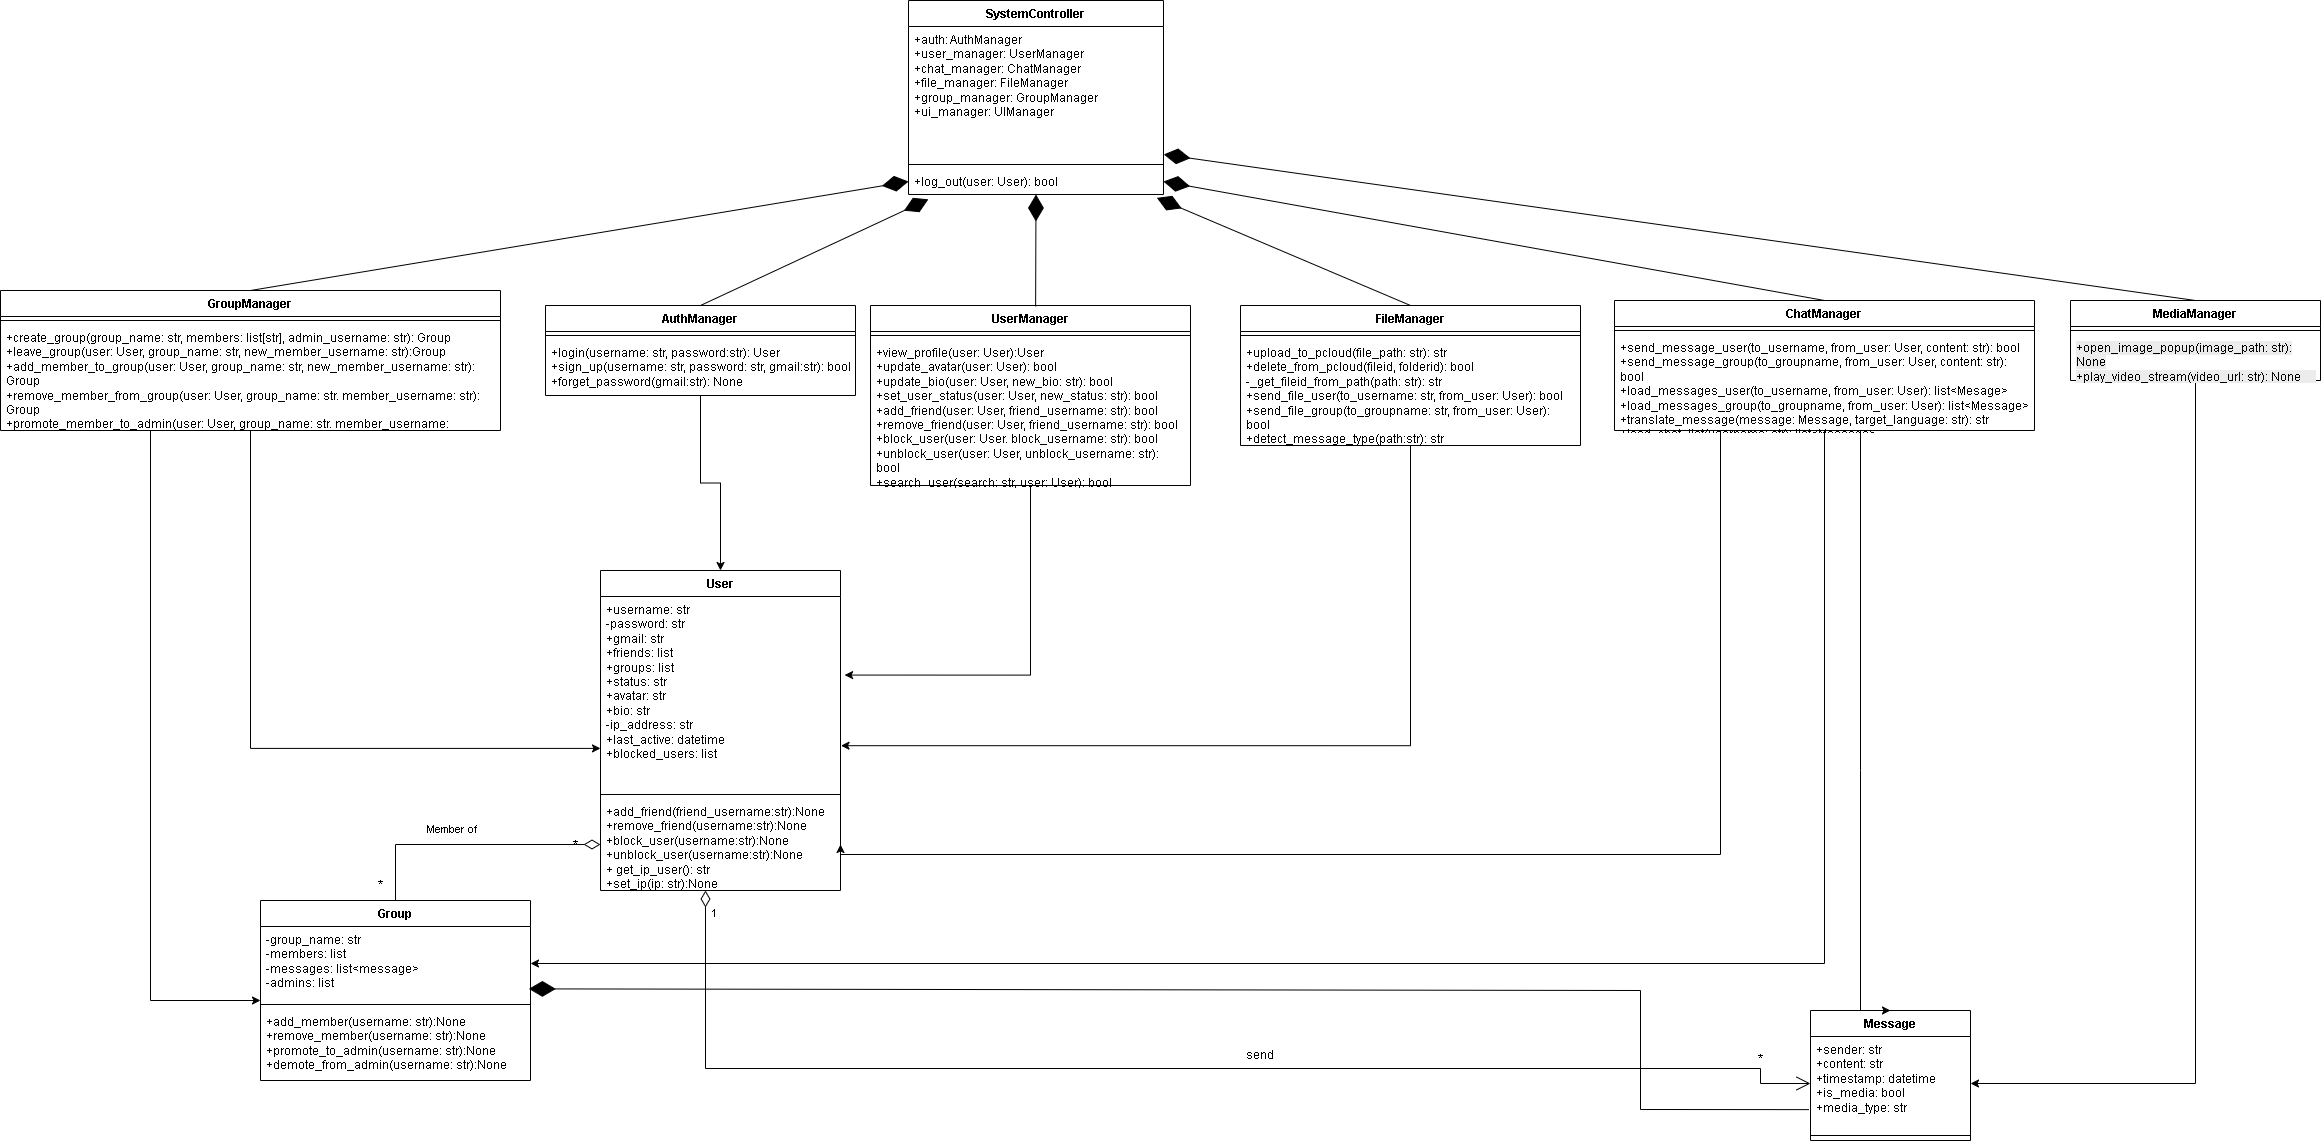
\includegraphics[angle=-90, width=0.45\textheight, keepaspectratio]{Class Diagram.png}
		
		\caption{Class Diagram (\href{https://drive.google.com/file/d/1nezddZGSJjMZVLKVG1fzco0IVRUCUjuZ/view}{Xem ảnh gốc tại đây})}
		\label{fig:class-diagram}
	\end{figure}
	
	
	\newpage
	
	%%%%%%%%%%%%%%%%%%%%%%%%%%%%%%%%%%%%%%%
	%%%%%%% Architectural Design %%%%%%%%%%
	%%%%%%%%%%%%%%%%%%%%%%%%%%%%%%%%%%%%%%%
	
	\section{Architectural Design}
	\subsection{Database Design}
	\subsubsection{ER Diagram}
	\begin{figure}[H]
		\centering
		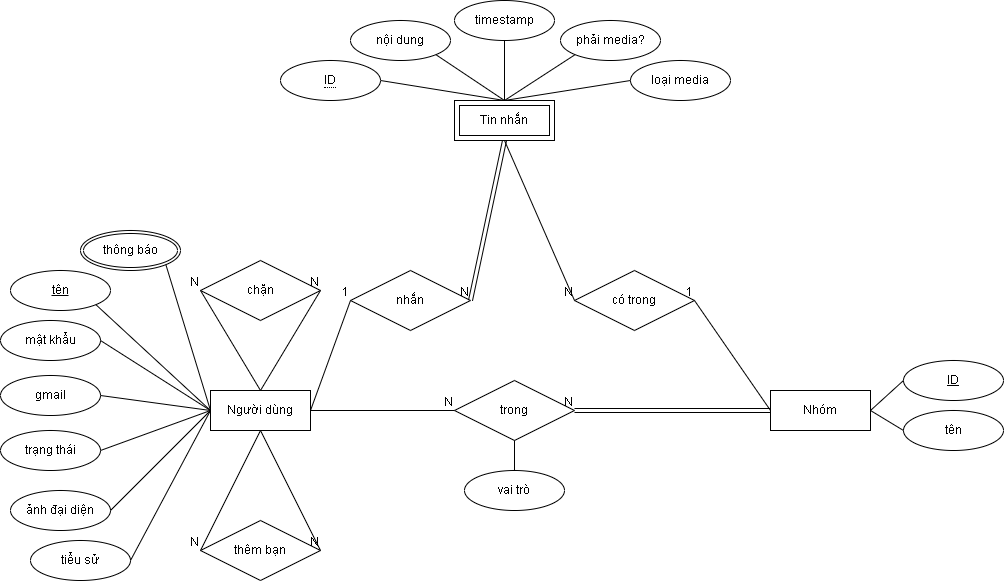
\includegraphics[width=1\textwidth]{ERD.png}    
		\caption{ER Diagram (\href{https://drive.google.com/file/d/1iTuhR-Tqn6hWHqBvqlqoMFTRaMn-1BZq/view?usp=drive_link}{Xem ảnh gốc tại đây})}
		\label{fig:hinh-minh-hoa}
	\end{figure} 
	\subsubsection{Database Schema}
	\begin{figure}[H]
		\centering
		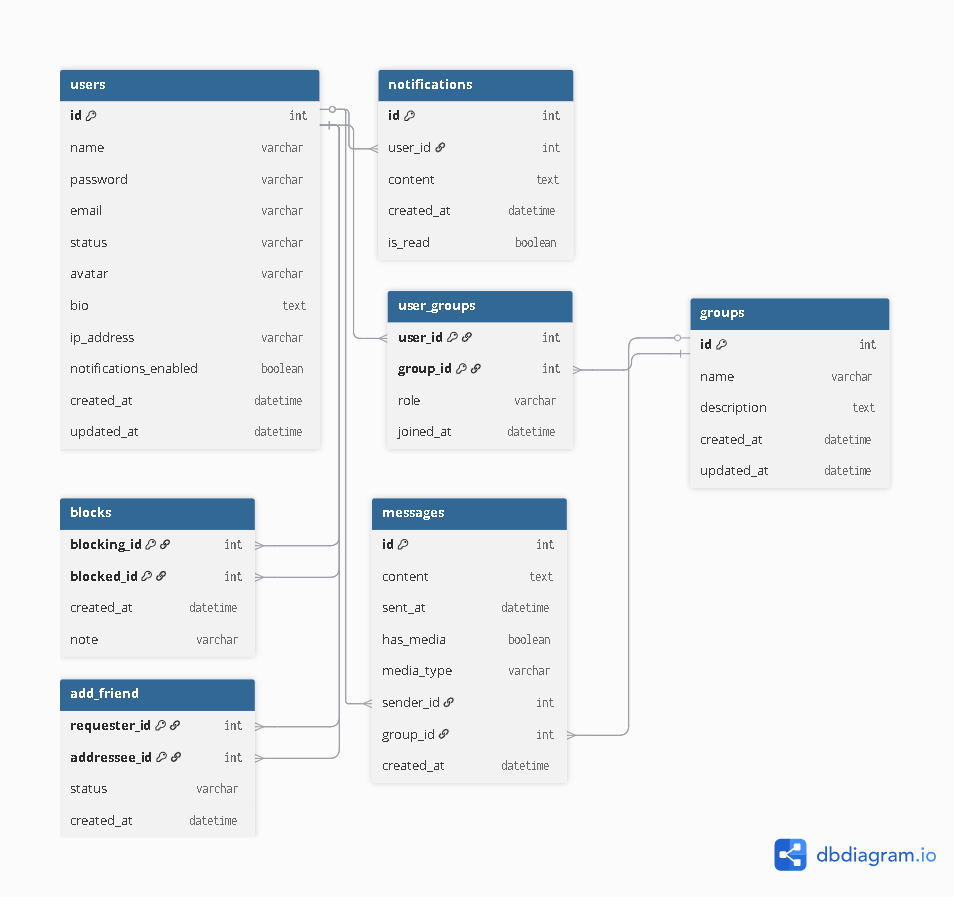
\includegraphics[width=1\textwidth]{Data Schema.png}    
		\caption{Relational Database Schema  (\href{https://dbdiagram.io/d/251_term_DATHCNPM_Schema-6902e2416735e11170697dc3}{Xem ảnh gốc tại đây})}
		\label{fig:hinh-minh-hoa}
	\end{figure} 
	
	\newpage
	\subsection{Software Architecture}
	\subsubsection{High-level Architecture}
	%...
	
	
	\subsubsection{Component Diagram}
	\begin{figure}[H]
		\centering
		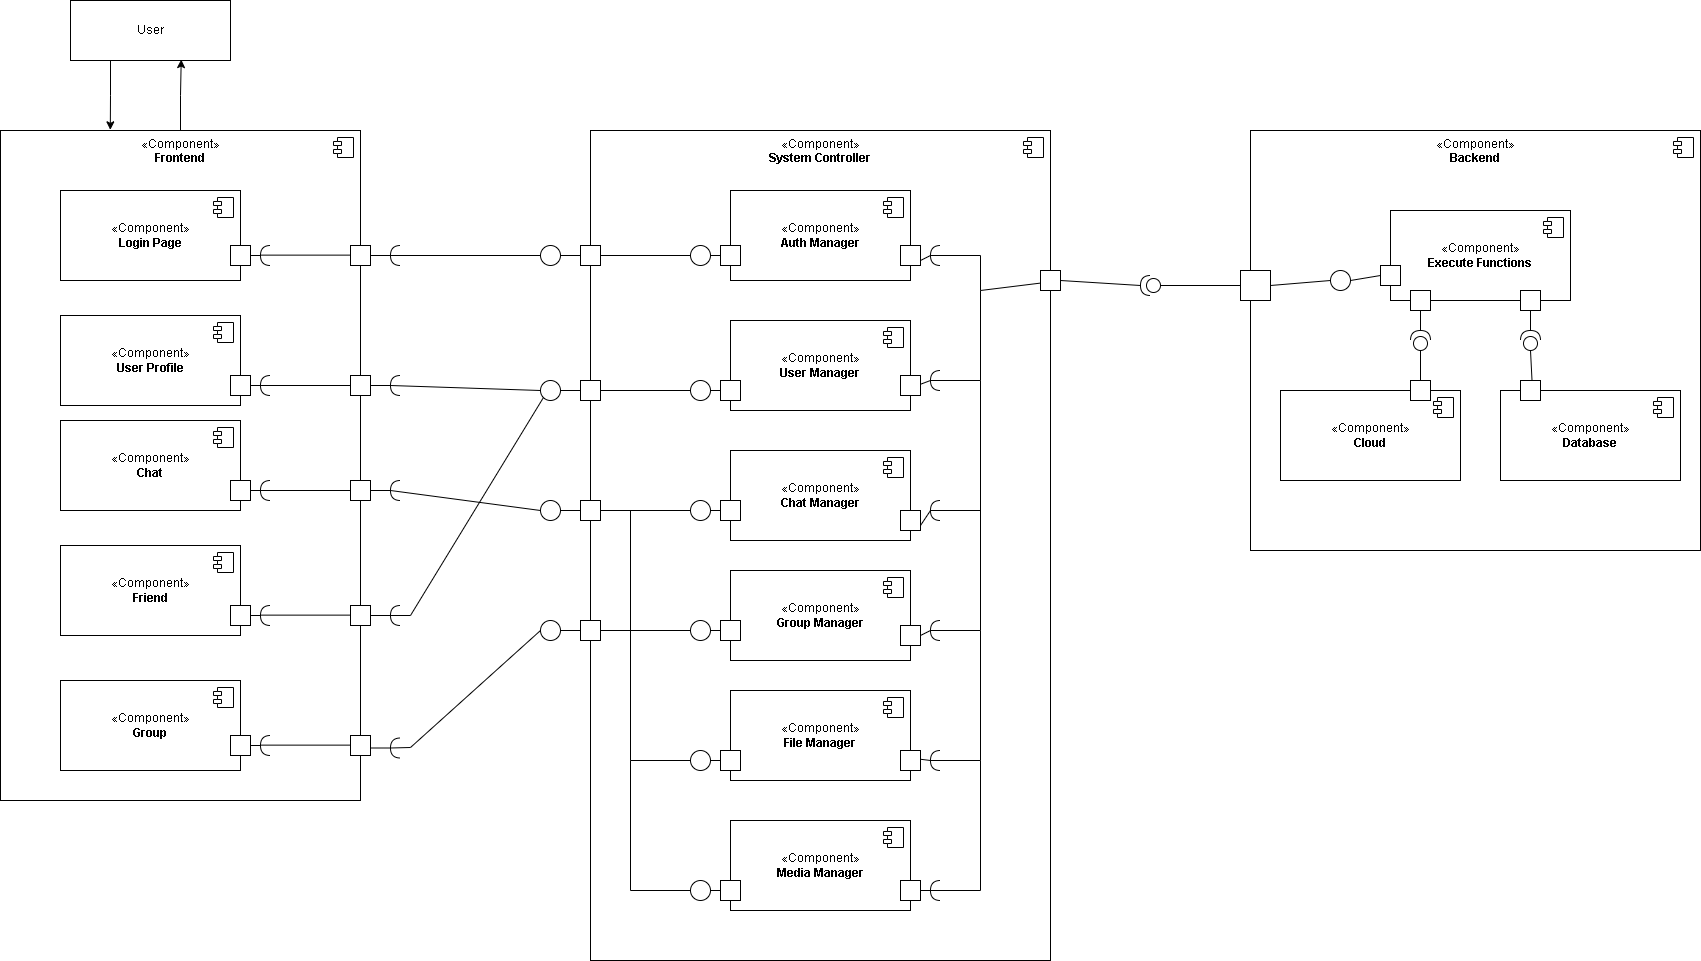
\includegraphics[width=1\textwidth]{Component Diagram}    
		\caption{Component Diagram (\href{https://drive.google.com/file/d/1rXUVUx75f55IQ1NsC87TX82kMlrD7k0V/view?usp=drive_link}{Xem ảnh gốc tại đây})}
		\label{fig:hinh-minh-hoa}
	\end{figure} 
	\subsubsection{Deployment Diagram}
	\begin{figure}[H]
		\centering
		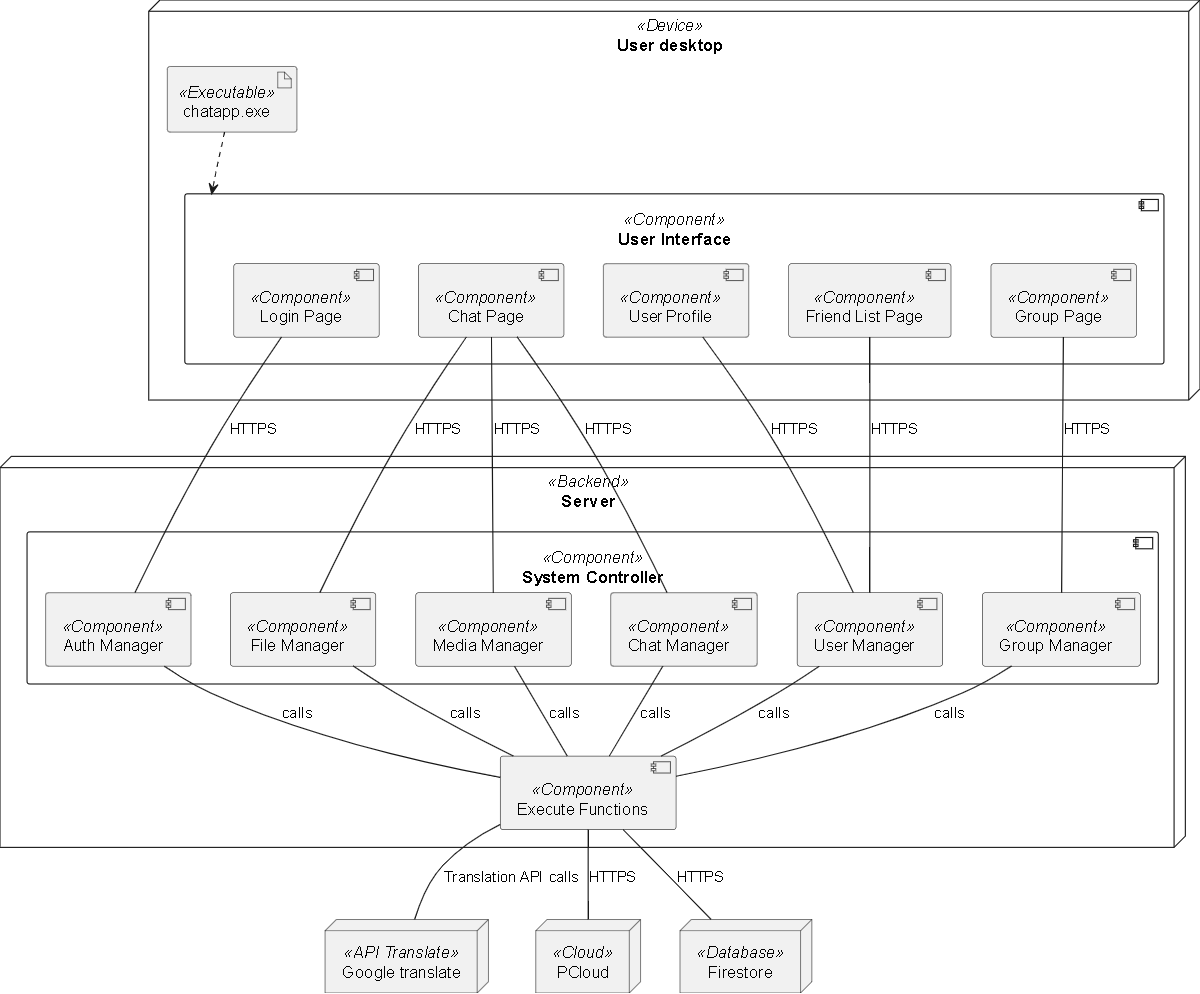
\includegraphics[width=1\textwidth]{Deployment Diagram}    
		\caption{Deployment Diagram (\href{https://drive.google.com/file/d/1rXUVUx75f55IQ1NsC87TX82kMlrD7k0V/view?usp=drive_link}{Xem ảnh gốc tại đây})}
		\label{fig:hinh-minh-hoa}
	\end{figure} 
\end{document}